\chapter{Phonologie}

\label{sec:phonologie}

Die im letzten Kapitel besprochene artikulatorische Phonetik lieferte eine Beschreibung der physiologischen Grundlagen der Sprachproduktion.
Anhand des Vorrats an Zeichen im IPA-Alphabet haben wir außerdem definiert, welche Laute im in Deutschland gesprochenen Standarddeutschen vorkommen.
Die eigentliche Frage der systematischen Grammatik bezüglich der Lautgestalt von Wörtern und größeren Einheiten ist aber, nach welchen Regularitäten die Segmente verbunden werden, und welchen Stellenwert die einzelnen Segmente und Segmentverbindungen (wie \zB Silben) im gesamten Lautsystem haben.
In der Phonologie geht es daher um das \textit{Lautsystem} und seine Regularitäten.
In Abschnitt~\ref{sec:segmente} wird der Status einzelner Laute und ihrer Vorkommen behandelt.
Es wird diskutiert, wie Laute im Lexikon gespeichert werden können, und schließlich werden einige konkrete phonologische Strukturbedingungen des Deutschen (wie die Auslautverhärtung) systematisch dargestellt.
Dann folgt eine recht ausführliche Analyse des \textit{Silbenbaus} (Abschnitt~\ref{sec:silbenundwoerter}).
Abschließend gibt Abschnitt~\ref{sec:wortakzent} einen Einblick in die \textit{Prosodie} (die \textit{Betonungslehre}) und damit in phonologische Aspekte auf Wortebene.

\section{Segmente}

\label{sec:segmente}

\subsection{Segmente und Verteilungen}

\label{sec:segmentemerkmaleverteilungen}

Der zentrale Begriff in der Phonologie ist zunächst wie in der Phonetik der des \textit{Segments}, vgl.\ Definition~\ref{def:segment}.\index{Segment}
Alternativ findet man auch den Begriff des \textit{Phonems}, auf den in Vertiefung~\ref{vert:phonephoneme} kurz eingegangen wird.
Allerdings geht es in der Phonologie anders als in der Phonetik um den systematischen Stellenwert der Segmente, nicht um eine reine Beschreibung ihrer Lautgestalt.
Um sich den Übergang von der Phonetik zur Phonologie klar zu machen, ist der Begriff der \textit{Verteilung} hilfreich.\index{Verteilung}
Schon in Abschnitt~\ref{sec:auslautverhaertungphonetik} wurde diskutiert, dass es bestimmte Positionen im Wort und in der Silbe gibt, an denen nur bestimmte Segmente vorkommen.
In jenem Abschnitt ging es zunächst lediglich um die Illustration einiger Beziehungen zwischen Schrift und Phonetik, aber in der Phonologie sind solche Phänomene von hohem theoretischen Stellenwert.
Das Beispiel war die Auslautverhärtung, die dazu führt, dass in der letzten Position der Silbe Obstruenten immer stimmlos sind (\textit{Bad} als \textipa{[ba:t]} und nicht *\textipa{[ba:d]}).
Man muss nun aber dennoch davon ausgehen, dass die betreffenden Wörter systematisch gesehen -- und vor allem im Lexikon -- einen stimmhaften Plosiv an der entsprechenden Stelle enthalten, denn wenn (\zB in Flexionsformen) ein weiterer Vokal folgt, ist der Plosiv stimmhaft, vgl.\ \textit{Bades} \textipa{[ba:d@s] nicht *\textipa{[ba:t@s]}}.
Ausgehend von dem Begriff der \textit{Verteilung} oder \textit{Distribution} (Definition~\ref{def:verteilung}) kann man in der Phonologie systematisch über solche Phänomene sprechen.

\Definition{Verteilung (Distribution)}{\label{def:verteilung}%
Die \textit{Verteilung} eines Segments ist die Menge der Umgebungen, in denen es vorkommt.
\index{Verteilung}
}

Die Beschreibung der Verteilung eines Segments nimmt typischerweise Bezug auf bestimmte Positionen in der Silbe oder im Wort, oder auf Positionen vor oder nach anderen Segmenten.
Es stellt sich damit die entscheidende Frage, ob zwei Segmente die \textit{gleiche Verteilung} oder eine \textit{teilweise} bzw.\ \textit{vollständig unterschiedliche Verteilung} haben.
Die Beispiele in (\ref{ex:phol6438})--(\ref{ex:phol6440}) illustrieren drei Typen von Verteilungen anhand des Vergleiches von je zwei Segmenten.

\begin{exe}
  \ex\label{ex:phol6438}
    \begin{xlist}
      \ex{\label{ex:phol6438a} Tod \textipa{[to:t]}, Kot \textipa{[ko:t]}}
      \ex{\label{ex:phol6438b} Schott \textipa{[SOt]}, Schock \textipa{[SOk]}}
    \end{xlist}
  \ex{\label{ex:phol6439} Hang \textipa{[haN]}, *\textipa{[Nah]}}
  \ex\label{ex:phol6440}
    \begin{xlist}
      \ex{\label{ex:phol6440a} Sog \textipa{[zo:k]}, besingen \textipa{[b@zIN@n]}, *\textipa{[so:k]}}
      \ex{\label{ex:phol6440b} fließ \textipa{[fli:s]}, Boss \textipa{[bOs]}, *\textipa{[fli:z]}}
      \ex{\label{ex:phol6440c} heißer \textipa{[h\t{aE}s5]}, heiser \textipa{[h\t{aE}z5]}, Base \textipa{[ba:z@]}, Basse \textipa{[bas@]}, *\textipa{[baz@]}}
    \end{xlist}
\end{exe}

(\ref{ex:phol6438}) zeigt, dass \textipa{[t]} und \textipa{[k]} eine (bezüglich ihrer Positionen in der Silbe) vollständig übereinstimmende Verteilung haben.
Sie kommen beide am Anfang und am Ende von Silben vor.
Hingegen haben \textipa{[h]} und \textipa{[N]} eine vollständig unterschiedliche  Verteilung, wie (\ref{ex:phol6439}) zeigt:
Am Anfang einer Silbe kommt nur \textipa{[h]} vor, am Ende einer Silbe kommt nur \textipa{[N]} vor.
Schließlich demonstriert (\ref{ex:phol6440}), dass \textipa{[s]} und \textipa{[z]} eine teilweise übereinstimmende Verteilung haben.
Am Anfang der ersten Silbe eines Wortes kommt nur \textipa{[z]} vor wie in (\ref{ex:phol6440a}), am Ende der letzten Silbe eines Wortes kommt nur \textipa{[s]} vor wie in (\ref{ex:phol6440b}).
Am Anfang einer Silbe in der Wortmitte kommen beide vor, \textipa{[z]} aber nur nach langem Vokal oder Diphthong wie in (\ref{ex:phol6440c}).

Wie man an den Beispielen sieht, gibt es Paare von Segmenten, anhand derer Wörter (wie \textit{heißer} und \textit{heiser}) unterschieden werden können, auch wenn die Wörter ansonsten völlig gleich lauten.
Dies funktioniert genau deshalb, weil die zwei Segmente jeweils mindestens eine teilweise übereinstimmende Verteilung haben.
Zwei Wörter, die sich nur in einem Segment an derselben Position unterscheiden, nennt man \textit{Minimalpaar}, und ein Minimalpaar illustriert jeweils einen \textit{phonologischen Kontrast}, s.\ Definition~\ref{def:phokonseg}.\index{Minimalpaar}


\Definition{Phonologischer Kontrast}{\label{def:phokonseg}%
Zwei phonetisch unterschiedliche Segmente bzw.\ Merkmale stehen in einem \textit{phonologischen Kontrast}, wenn sie eine teilweise oder vollständig übereinstimmende Verteilung haben und dadurch einen lexikalischen bzw.\ grammatischen Unterschied markieren können.
\index{Kontrast}
}

Ein phonologischer Kontrast besteht \zB zwischen \textipa{[t]} und \textipa{[k]}, weil wir Wörter anhand dieser Segmente unterscheiden können.
Das Gleiche gilt für \textipa{[s]} und \textipa{[z]} und viele andere Paare von Segmenten.
Es gilt aber nicht für \textipa{[h]} und \textipa{[N]}, weil diese beiden Segmente keine übereinstimmende Verteilung haben, wie in (\ref{ex:phol6439}) gezeigt wurde.
Diese Art der Verteilungen nennt man \textit{komplementär}, vgl.\ Definition~\ref{def:komplementaer}.

\Definition{Komplementäre Verteilung}{\label{def:komplementaer}%
Eine \textit{komplementäre Verteilung} zweier Segmente liegt dann vor, wenn die beiden Segmente in keiner gemeinsamen Umgebung vorkommen.
Komplementär verteilte Segmente können prinzipiell keinen phonologischen Kontrast markieren.
\index{Verteilung!komplementär}
}

Über Verteilungen lässt sich schon anhand des bisher eingeführten Inventars von Beispielen noch mehr sagen.
Bei der bereits besprochenen Auslautverhärtung haben wir es mit Paaren von stimmlosen und stimmhaften Plosiven zu tun, die in bestimmten Umgebungen (im Silbenanlaut) einen Kontrast markieren, der aber in anderen Umgebungen (Silbenauslaut) verschwindet.\index{Auslautverhärtung}
(\ref{ex:phol-5674-1})--(\ref{ex:phol-5674-3}) zeigen dies für \textipa{[g]} und \textipa{[k]}, \textipa{[d]} und \textipa{[t]} sowie \textipa{[b]} und \textipa{[p]}.

\begin{exe}
  \ex\label{ex:phol-5674-1}
  \begin{xlist}
    \ex{Weg \textipa{[ve:k]}, Weges \textipa{[ve:g@s]}}
    \ex{Bock \textipa{[bOk]}, Bockes \textipa{[bOk@s]}}
  \end{xlist}
  \ex\label{ex:phol-5674-2}
  \begin{xlist}
    \ex{Bad \textipa{[ba:t]}, Bades \textipa{[ba:d@s]}}
    \ex{Blatt \textipa{[blat]}, Blattes \textipa{[blat@s]}}
  \end{xlist}
  \ex\label{ex:phol-5674-3}
  \begin{xlist}
    \ex{Lob \textipa{[lo:p]}, Lobes \textipa{[lo:b@s]}}
    \ex{Depp \textipa{[dEp]}, Deppen \textipa{[dEp@n]}}
  \end{xlist}
\end{exe}

Im Silbenauslaut des Deutschen gibt es prinzipiell keinen Unterschied zwischen stimmlosen und stimmhaften Plosiven.
Solche Effekte nennt man \textit{Neutralisierungen}, s.\ Definition~\ref{def:neutralisierung}.

\Definition{Neutralisierung}{\label{def:neutralisierung}%
Eine \textit{Neutralisierung} ist die Aufhebung eines phonologischen Kontrasts in einer bestimmten Position.
\index{Neutralisierung}
}

Im Silbenauslaut wird im Deutschen also der phonologische Kontrast zwischen \textipa{[g]} und \textipa{[k]}, zwischen \textipa{[d]} und \textipa{[t]} usw.\ neutralisiert.
Allgemein gesprochen wird der Kontrast zwischen stimmlosen und stimmhaften Plosiven (vgl.\ Abschnitt~\ref{sec:stimmhaftigkeit}) in dieser Position neutralisiert.
Daher ist in Definition~\ref{def:phokonseg} von zwei phonetisch unterschiedlichen Segmenten bzw.\ \textit{Merkmalen} die Rede.
Phonologische Kontraste bestehen im Prinzip zwischen Merkmalen und erst in zweiter Ordnung zwischen ganzen Segmenten.

Das Feststellen von Verteilungen ist allerdings kein Selbstzweck.
Durch die Untersuchung aller Verteilungen in einer Sprache konstruiert man das phonologische System (die phonologische Komponente der Grammatik).
Dabei geht es darum, die Formen zu ermitteln, die im Lexikon gespeichert werden müssen, und die Strukturbedingungen (wie die Auslautverhärtung) zu beschreiben, an die die Segmente in diesen Formen ggf.\ angepasst werden müssen.
Die \textit{lexikalisch gespeicherten} bzw.\ \textit{zugrundeliegenden Formen} und die \textit{phonologischen Strukturbedingungen} produzieren die konkreten phonetischen Verteilungen an der Oberfläche.

\subsection{Zugrundeliegende Formen und Strukturbedingungen}

\label{sec:zugrundeliegendeformenstrukturbedingungen}

Wir bleiben jetzt beim Beispiel der Auslautverhärtung, um die Idee von lexikalisch zugrundeliegenden Formen und phonologischen Strukturbedingungen einzuführen.
Die Auslautverhärtung hat wie erwähnt zur Folge, dass für Obstruenten im Silbenauslaut der Stimmtonkontrast neutralisiert wird, denn alle Obstruenten im Silbenauslaut sind stimmlos.
Wenn man das gesamte Paradigma der Wörter in (\ref{ex:phol-5674-1})--(\ref{ex:phol-5674-3}) ansieht, fällt aber dennoch ein bedeutender Unterschied auf.
In manchen Wörtern steht im Silbenauslaut ein Konsonant, der in anderen Umgebungen stimmhaft ist, wie in \textipa{[ve:k]} und \textipa{[ve:g@s]}.
In anderen Wörtern steht ein stimmloser Konsonant, der auch in diesen anderen Umgebungen stimmlos bleibt, wie in \textipa{[bOk]} und \textipa{[bOk@s]}.
Es ist daher naheliegend, anzunehmen, dass Wörter wie \textit{Weg} (oder \textit{Bad}, \textit{Lab} usw.) eine \textit{zugrundeliegende Form} haben, in der der letzte Obstruent stimmhaft ist.
Diese zugrundeliegende Form ist eine der wesentlichen Informationen, die zum \textit{lexikalischen Wort} gehören (vgl.\ Abschnitt~\ref{sec:woerterwortformen}).

Die eigentliche Grammatik stellt allerdings allgemeine Anforderungen an die Wohlgeformtheit von Strukturen, hier die \textit{phonologischen Strukturbedingungen}.
Der \textit{Prozess} der Auslautverhärtung (als Veränderung der Merkmale eines Segments) ist in diesem Sinn das Ergebnis einer Anpassung von Silben an die Strukturbedingung, dass Silben nicht auf stimmhafte Obstruenten enden können.%
\footnote{Man kann die phonologische Grammatik in Form von \textit{Prozessen} bzw.\ \textit{Regeln} (im technischen Sinne) formulieren, die Formen als Eingabematerial nehmen und modifiziert als Ausgabematerial wieder ausgeben.\index{phonologischer Prozess}
Die Auslautverhärtung wäre dann einfach eine Regel in diesem technischen Sinn.
Alternativ kann man davon ausgehen, dass eine phonologische Grammatik aus Beschreibungen zulässiger Strukturen besteht, an die konkrete Formen angepasst werden.
Wie diese Anpassung vor sich geht, ist auch wieder eine sehr technische Frage.
Innerhalb einer phonembasierten Theorie (Vertiefung~\ref{vert:phonephoneme}) bieten sich wieder andere Möglichkeiten, die Beziehung von Formen und Strukturbedingungen zu erfassen.
Die technischen Unterschiede sind für unsere Zwecke mehr als nachrangig.
Eine deskriptive Grammatik ist wahrscheinlich am besten bedient, wenn sie sich darauf beschränkt, zu beschreiben, wie Formen im Lexikon und an der Oberfläche aussehen, also systematische Beziehungen -- eben \textit{Regularitäten} (Abschnitt~\ref{sec:regulgen}) -- feststellt.}
Die zugrundeliegende Form muss also genau die Informationen zu einem Wort enthalten, die ausreichen, um seine lautliche Gestalt in allen möglichen Formen und Umgebungen ableiten zu können.
Definition~\ref{def:pholproz} fasst zusammen.


\Definition{Zugrundeliegende Form und Strukturbedingung}{\label{def:pholproz}%
Die \textit{zugrundeliegende Form} (eines Wortes) ist genau die Folge von Segmenten, die im Lexikon gespeichert wird, und auf die alle zugehörigen phonetischen Formen zurückgeführt werden können.
Die Formen werden ggf. an die phonologischen \textit{Strukturbedingungen} (die Regularitäten der phonologischen Grammatik) angepasst.
\index{zugrundeliegende Form}
\index{Strukturbedingung}
\index{Lexikon}
}

Neben der Auslautverhärtung ist ein anderes illustratives Beispiel für zugrundeliegende Formen und Strukturbedingungen die Einfügung des Glottalplosivs.\index{Glottalverschluss}
Wie in Abschnitt~\ref{sec:laryngale} bereits besprochen, steht im Deutschen am Wortanfang und vor betonten Silben innerhalb von Wörtern stets ein Konsonant.
In scheinbar vokalisch anlautenden Wörtern wie \textit{Ort} oder \textit{Insel} wird der laryngale Plosiv oder Glottalverschluss \textipa{[P]} eingefügt.
Man artikuliert \textipa{[P\t{O@}t]} und \textipa{[PInz@l]}.
Ein Beispiel für dasselbe Phänomen vor einer betonten Silbe innerhalb eines Wortes ist das Wort \textit{Verein}, das \textipa{[f5P\t{aE}n]} artikuliert wird.
Wir haben es also mit einer Strukturbedingung für die Form von Silben und Wörtern zu tun.
Zugrundeliegend muss \textipa{[P]} damit nicht spezifiziert werden, weil nur durch seine An- bzw.\ Abwesenheit niemals zwei Wörter unterschieden werden können.
Es gibt also aus systematischen Gründen keine Minimalpaare.
\textit{Asche} \textipa{[PaS@]} und \textit{Tasche} \textipa{[taS@]} sind zwei verschiedene Wörter und im Prinzip ein Minimalpaar.
Weil die Anwesenheit des Glottalverschlusses aber vollständig vorhersagbar ist und er in den Umgebungen, in denen er auftritt, nicht weggelassen werden kann, ist *\textipa{[aS@]} unmöglich.
Genau deswegen bilden *\textipa{[aS@]} und \textipa{[PaS@]} auch kein Minimalpaar.

Ein andere Art der Reduktion wird später für auslautendes \textipa{[N]} vorgenommen.
Einerseits ist \textipa{[N]} die Vertretung für \textipa{[n]} vor velaren Plosiven wie in \textit{Bänke} \textipa{[bENk@]}.
In diesen Fällen liegt es nah, davon auszugehen, dass sich der Nasal an den Plosiv in seinem Artikulationsort anpasst.
Andererseits tritt das Segment auch einzeln am Silbenende auf, wie in \textit{Gang} \textipa{[gaN]}.
Man kann \textipa{[N]} auch in diesen Fällen phonologisch auf eine zugrundeliegende Folge von \textipa{[n]} und \textipa{[g]} zurückführen (s.\ Abschnitt~\ref{sec:systematikderraender}).

Die Phonologie stellt also eine Abstraktion gegenüber der Phonetik dar.\index{Phonologie}
Die Phonetik eines Wortes beschreibt, wie es tatsächlich ausgesprochen wird, und jedes einzelne Wort einer Sprache kann ohne Betrachtung der anderen Wörter phonetisch beschrieben werden.
Die phonologische Repräsentation eines Wortes erfordert hingegen zusätzliches Wissen um Strukturbedingungen (\zB in Form der Auslautverhärtung), um aus ihr phonetische Formen abzuleiten.
Dieses Wissen erschließt sich durch die Betrachtung des gesamten Sprachsystems, also jedes Wortes in Bezug zu allen anderen Wörtern und in allen möglichen Umgebungen.
Anders gesagt müssen die \textit{Verteilungen der Segmente} bekannt sein.

\begin{table}[!htbp]
  \resizebox{\textwidth}{!}{
    \begin{tabular}{ccc}
      \lsptoprule
      \multicolumn{2}{c}{\textbf{Grammatik}} & \textbf{Externe Systeme} \\
      \midrule
      \textbf{Lexikon} & \textbf{Phonologie} & \textbf{Phonetik} \\
      \midrule
      /~/& $\Rightarrow$ & \textipa{[~]}\\
      zugrundeliegende Form & Anpassung an Strukturbedingungen & phonetische Realisierung \\
      \lspbottomrule
    \end{tabular}
  }
  \caption{Lexikon, Phonologie und Phonetik}
  \label{tab:pholsystem}
\end{table}
\index{Lexikon}

Zugrundeliegende phonologische Formen schreibt man konventionellerweise nicht in \textipa{[~]}, sondern in /~/, also \zB /\textipa{veg}/, /\textipa{bad}/ und /\textipa{lab}/ oder /\textipa{OKt}/ und \mbox{/\textipa{Inz@l}/}.%
\footnote{Warum die Länge in /~/ nicht notiert wird, wird in Abschnitt~\ref{sec:gespanntheitbetonunglaenge} erläutert.}
Schematisch kann man die Verhältnisse wie in Tabelle~\ref{tab:pholsystem} darstellen.
Mit \textit{externen Systemen} sind nicht zur Grammatik gehörige Systeme wie Gehör und Sprechapparat gemeint.
In den Abschnitten~\ref{sec:auslautverhaertungphonologie} bis~\ref{sec:rvokalisierungen} werden beispielhaft einige Strukturbedingungen und Verteilungen besprochen, um zu illustrieren, wie ein phonologisches System konstruiert werden kann.
Dabei ist es manchmal nicht trivial, zu entscheiden, ob bestimmte Repräsentationen besser in /~/ oder [~] stehen sollten.
Wir tendieren dazu, [~] im Zweifelsfall den Vorzug zu geben.

\subsection{Auslautverhärtung}

\label{sec:auslautverhaertungphonologie}
\index{Auslautverhärtung}

Die Auslautverhärtung lässt sich als Strukturbedingung unter Bezug auf phonetische bzw.\ phonologische Merkmale (Abschnitt~\ref{sec:phonetischemerkmale}), bestimmte Positionen in Wort oder Silbe und die Oberklassen für Segmente (Abschnitt~\ref{sec:oberklassenfuerartikulationsarten}) sehr einfach und kompakt mit Satz~\ref{satz:auslautverhaertung} beschreiben.

\Satz{Auslautverhärtung}{\label{satz:auslautverhaertung}Segmente mit [\textsc{Obstruent}:~$+$] sind am Silbenende [\textsc{Stimme}:~$-$].}

Wenn wir zugrundeliegende Formen an diese Bedingung anpassen wollen, muss also die Silbenstruktur bekannt sein.
Um diese geht es in Abschnitt~\ref{sec:silben} noch im Detail, hier werden die Silbengrenzen einfach vorgegeben und durch Punkte markiert.
Nur zur Veranschaulichung steht \phopro\ für \textit{wird phonetisch  realisiert als}.%
\footnote{In (\ref{ex:phol6726a}) ist \textit{Bad} standardkonform mit langem \textipa{[a:]} notiert.
Die Variante mit kurzem \textipa{[a]} (also \textipa{[bat]}) ist regional.}

\begin{exe}
  \ex\label{ex:phol6726}
  \begin{xlist}
    \ex{\label{ex:phol6726a} /\textipa{bad}/ \phopro \textipa{[ba:t]}}
    \ex{\label{ex:phol6726b} /\textipa{bad@s}/ \phopro \textipa{[ba:.d@s]}}
    \ex{\label{ex:phol6726c} /\textipa{bat}/ \phopro \textipa{[ba:t]}}
  \end{xlist}
\end{exe}

Abhängig von der zugrundeliegenden Form und der Silbenstruktur muss eine Veränderung stattfinden -- oder eben nicht.
In (\ref{ex:phol6726a}) steht /\textipa{d}/ am Silbenende und ist zugrundeliegend mit [\textsc{Stimme}: $+$] spezifiziert.
Weil /\textipa{d}/ den Wert [\textsc{Obstruent}: $+$] hat, wird der Wert des Stimmton-Merkmals auf [\textsc{Stimme}: $-$] gesetzt.
In (\ref{ex:phol6726b}) ist die Silbenstruktur anders, die Bedingung für die Auslautverhärtung ist nicht erfüllt, und die Form bleibt unverändert.
In (\ref{ex:phol6726c}) steht zwar ein Obstruent /\textipa{t}/ am Silbenende, aber es muss keine Anpassung stattfinden, weil /\textipa{t}/ von vornherein [\textsc{Stimme}: $-$] ist.

\subsection{Gespanntheit, Betonung und Länge}

\label{sec:gespanntheitbetonunglaenge}

\index{Vokal!Länge}
\index{Vokal!Gespanntheit}
Die Formulierung von Strukturbedingungen kann helfen, die Menge der Merkmale zu reduzieren, die man zugrundeliegend spezifizieren muss.
Anders gesagt kann man sich überlegen, ob die Werte für bestimmte Merkmale automatisch aus anderen Merkmalen und den Positionen der jeweiligen Segmente vorhergesagt werden können.
Solche Reduktionen sind typisch für die Phonologie im Gegensatz zur Phonetik, weil eine einfache Systembeschreibung aus allgemeinen wissenschaftlichen Ökonomiegründen einer komplexeren vorzuziehen ist.

In Abschnitt~\ref{sec:phonetischemerkmale} wurde die Vokallänge als gewöhnliches Merkmal (\textsc{Lang}) eingeführt.
Gleichzeitig wurde festgestellt, dass nur die Vokale \textipa{[i]}, \textipa{[y]}, \textipa{[u]}, \textipa{[e]}, \textipa{[\o]}, \textipa{[E]}, \textipa{[o]} und \textipa{[a]} lange und kurze Varianten haben.
Bezüglich der Akzentuierung bzw.\ Betonung ist ebenfalls bereits bekannt, dass alle Vokale bis auf \textipa{[@]} und \textipa{[5]} betonbar sind, und dass bei den Vokalen mit Längenunterschied die Länge an die Betonung gebunden ist.
Dieser Abschnitt verfolgt nun zwei Ziele.
Erstens wird das Merkmal \textsc{Gespannt} vorgeschlagen, um genau diejenigen Vokale zusammenzufassen, die sowohl lang als auch kurz vorkommen.
Zweitens wird dadurch das Merkmal \textsc{Lang} aus allen zugrundeliegenden Formen eliminiert, und das Merkmal \textsc{Lage} wird auf drei Werte reduziert.
Wir führen also zunächst das Merkmal \textsc{Gespannt} ein und spezifizieren es zugrundeliegend als [\textsc{Gespannt}: $+$] für die oben genannten Vokale, die lange und kurze Varianten haben.
In (\ref{ex:phol91919166}) wird das Merkmal deklariert.
Beispiel (\ref{ex:phol0118999}) zeigt die resultierende zugrundeliegende Spezifikation für /i/ und /\textipa{I}/.

\begin{exe}
  \ex{\label{ex:phol91919166}\textsc{Gespannt}: $+$, $-$}
  \ex\label{ex:phol0118999}
  \begin{xlist}
    \ex /i/ = [\textsc{Lage}: \textit{vorne}, \textsc{Höhe}: \textit{hoch}, \textsc{Gespannt}: $+$, \textsc{Rund}: $-$]
    \ex /\textipa{I}/ = [\textsc{Lage}: \textit{vorne}, \textsc{Höhe}: \textit{hoch}, \textsc{Gespannt}: $-$, \textsc{Rund}: $-$]
  \end{xlist}
\end{exe}

Es ergibt sich das neue Vokaltrapez in Abbildung~\ref{fig:vokalviereckmitgespannt}, das um den Preis erkauft wird, dass \textipa{[E]} und \textipa{[a]} jeweils bald als gespannt, bald als ungespannt angesehen werden.
Das gespannte \textipa{[a]} ist phonetisch nicht vom ungespannten \textipa{[a]} unterscheidbar, und Gleiches gilt für gespanntes und ungespanntes \textipa{[E]}.
In der phonologischen Notation schreiben wir hier /\textipa{\u{a}}/ und /\textipa{\u{E}}/ für die \textit{ungespannten} Varianten, um den Unterschied zu markieren.
Generell ist Abbildung~\ref{fig:vokalviereckmitgespannt} nicht streng phonetisch zu lesen, sondern als abstrakte phonologische Darstellung.
Phonetisch gilt weiterhin Abbildung~\ref{fig:vokaltrapneu} (S.~\pageref{fig:vokaltrapneu}).
Schwa und \textipa{[5]} fehlen hier, weil sie außerhalb des Systems der gespannten und ungespannten Vokale stehen (s.\,u.\ Satz~\ref{satz:schwabetont}).

\begin{figure}[!htpb]
  \centering
  \begin{tikzpicture}[scale=3.5,baseline=default]
    \large
    \tikzset{
    vowel/.style={fill=white, anchor=mid, text depth=0ex, text height=1ex},
    vowelgespannt/.style={circle,fill=gray!30, anchor=mid, text depth=0ex, text height=1ex,minimum size=4ex},
    dot/.style={circle,fill=black,minimum size=0.4ex,inner sep=0pt,outer sep=-1pt},
    }

    \coordinate (hf) at (0,2); % high front
    \coordinate (hb) at (2,2); % high back
    \coordinate (lf) at (1,0); % low front
    \coordinate (lb) at (2,0); % low back
    \def\V(#1,#2){barycentric cs:hf={(3-#1)*(2-#2)},hb={(3-#1)*#2},lf={#1*(2-#2)},lb={#1*#2}}

    % Chart key (vorne -- hinten).
    \draw [{Latex[round]}-] (\V (-.25,0)) -- (\V (-.25,.5))  node [above left] {\footnotesize vorne};
    \draw [-{Latex[round]}] (\V (-.25,1.5)) -- (\V (-.25,2)) node [above left] {\footnotesize hinten};
    \path (\V (-.25,1)) node[above] {\footnotesize zentral};

    % Chart key (hoch--tief).
    \draw [{Latex[round]}-] (\V (0,-.25)) -- +(270:.5cm)  node [above right,rotate=90] (vokaltrapez1) {\footnotesize hoch};
    \draw [{Latex[round]}-] (\V (3,-2.5)) -- +(270:-.5cm) node [above left,rotate=90] (vokaltrapez2) {\footnotesize tief};
    \path (\V (1.5,-1)) node[above,rotate=90] {\footnotesize mittel};

    % Grid.
    \draw [gray,thick] (\V(0,0)) -- (\V(0,2));
    \draw [gray,thick] (\V(3,0)) -- (\V(3,2));
    \draw [gray,thick] (\V(0,0)) -- (\V(3,0));
    \draw [gray,thick] (\V(0,2)) -- (\V(3,2));

    \path (\V(0,0))      node[vowelgespannt] (i)   {i};
    \path (\V(0.25,0))   node[vowelgespannt] (y)   {y};
    \path (\V(0.4,0.5))  node[vowel]         (ii)  {ɪ};
    \path (\V(0.65,0.5)) node[vowel]         (yy)  {ʏ};
    \path (\V(1,0))      node[vowelgespannt] (e)   {e};
    \path (\V(1.25,0))   node[vowelgespannt] (oe)  {ø};
    \path (\V(2,0))      node[vowelgespannt] (ee)  {ɛ};
    \path (\V(1.4,0.7))  node[vowel]         (eee) {ɛ̆};
    \path (\V(1.65,0.7)) node[vowel]         (oee) {œ};
    \path (\V(3,1))      node[vowelgespannt] (a)   {a};
    \path (\V(2.5,1))    node[vowel]         (aa)  {ă};
    \path (\V (1,2))     node[vowelgespannt] (o)   {o};
    \path (\V (1.5,1.4)) node[vowel]         (oo)  {ɔ};
    \path (\V (0,2))     node[vowelgespannt] (u)   {u};
    \path (\V (0.5,1.5)) node[vowel]         (uu)  {ʊ};

    \draw (i)  -- (ii);
    \draw (y)  -- (yy);
    \draw (e)  -- (eee);
    \draw (oe) -- (oee);
    \draw (ee) -- (eee);
    \draw (a)  -- (aa);
    \draw (o)  -- (oo);
    \draw (u)  -- (uu);
  \end{tikzpicture}
  \caption[Phonologisches Vokaltrapez]{Phonologisches Vokaltrapez (Grau für [\textsc{Gespannt}: $+$])}
  \label{fig:vokalviereckmitgespannt}
  \index{Vokaltrapez}
\end{figure}

Die Vokale in den ersten Silben von \textit{Liebe} \textipa{[li:b@]}, \textit{Tüte} \textipa{[ty:t@]}, \textit{Wut} \textipa{[vu:t]}, \textit{Weg} \textipa{[ve:k]}, \textit{schön} \textipa{[S\o:n]}, \textit{Käse} \textipa{[kE:z@]}, \textit{rot} \textipa{[Ko:t]}, \textit{rate} \textipa{[Ka:t@]} gelten also gemäß dieser leicht veränderten Merkmalsmenge als \textit{gespannt}.
In diesen Beispielen sind sie betont und daher lang.
Ungespannte Vokale können betont werden, aber sie werden dadurch nicht lang, \zB \textit{Rinder} \textipa{[KInd5]}.
Formen wie *\textipa{[KI:nd5]} sind ausgeschlossen.
Tabelle~\ref{tab:gespungesp} gibt einen systematischen Überblick in Form von Beispielen.

\begin{table}[!htbp]
  \centering
  \begin{tabular}{cllp{0.25cm}cll}
    \lsptoprule
    \textbf{gespannt} & \textbf{Beispiel} & \textbf{IPA} & & \textbf{ungespannt} & \textbf{Beispiel} & \textbf{IPA} \\
    \midrule
    \textipa{i}  & \textit{bieten} & \textipa{bi:t@n} && \textipa{I} & \textit{bitten}  & \textipa{bIt@n}   \\
    \textipa{y}  & \textit{fühlt}  & \textipa{fy:lt}  && \textipa{Y} & \textit{füllt}   & \textipa{fYlt}    \\
    \textipa{u}  & \textit{Mus}    & \textipa{mu:s}   && \textipa{U} & \textit{muss}    & \textipa{mUs}     \\
    \textipa{e}  & \textit{Kehle}  & \textipa{ke:l@}  && \textipa{E} & \textit{Kelle}   & \textipa{kEl@}    \\
    \textipa{E}  & \textit{stähle} & \textipa{StE:l@} && \textipa{E} & \textit{Ställe}  & \textipa{StEl@}   \\
    \textipa{\o} & \textit{Höhle}  & \textipa{h\o:l@} && \textipa{\oe} & \textit{Hölle} & \textipa{h\oe l@} \\
    \textipa{o}  & \textit{Ofen}   & \textipa{Po:f@n} && \textipa{O} & \textit{offen}   & \textipa{POf@n}   \\
    \textipa{a}  & \textit{Wahn}   & \textipa{va:n}   && \textipa{a} & \textit{wann}    & \textipa{van}     \\
    \lspbottomrule
  \end{tabular}
  \caption{Gespannte und ungespannte Vokale im Kernwortschatz}
  \label{tab:gespungesp}
\end{table}

Was Gespanntheit phonetisch auszeichnet, ist nicht einfach zu bestimmen.
Man kann versuchen, die Kategorie der Gespanntheit mit einer erhöhten Muskelanspannung oder einer Veränderung der Position der Zungenwurzel in Verbindung zu bringen.
Aus Sicht der Phonologie ist der \textit{systematische} Aspekt aber wichtiger als der artikulatorische.
Für die gespannten Vokale gelten gemeinsame Strukturbedingungen, und daher sollte sie die Grammatik idealerweise als eine Klasse von Segmenten auffassen -- genauso wie die stimmhaften und stimmlosen Obstruenten usw.
Mit den Ortsmerkmalen der Vokale und der Lippenrundung alleine könnte man die gespannten (und damit längbaren) Vokale aber nicht von den ungespannten unterscheiden.
Klassen definieren wir über Merkmale und Werte (vgl.\ Abschnitt~\ref{sec:merkmaleundwerte}), und daher ist das neue Merkmal gerechtfertigt.


Weil die halbvorderen und halbhinteren Vokale jetzt durch die Gespanntheit von den vorderen und hinteren unterscheidbar werden, kann ein weiteres Merkmal in seinen möglichen Werten reduziert werden.

\begin{exe}
  \ex \textsc{Lage}: \textit{vorne}, \textit{zentral}, \textit{hinten}
\end{exe}

Je nach Auffassung, was der Kernwortschatz ist, gilt im Kernwortschatz (auf jeden Fall aber im Erbwortschatz), dass gespannte Vokale immer betont und damit immer lang sind.%
\footnote{Zum Kernwortschatz und Erbwortschatz s.\ Abschnitt~\ref{sec:kernundperipherie}.}
Innerhalb des Kernwortschatzes gibt es damit die in Abbildung~\ref{fig:vokalviereckmitgespannt} durch Striche verbundenen Paare aus langen gespannten betonten und kurzen ungespannten betonten oder unbetonten Vokalen.
Während die ungespannten betont oder unbetont auftreten können, sind die gespannten immer betont, vgl.\ Satz~\ref{satz:gespanntheitkern}.

\Satz{Gespanntheit im Kernwortschatz}{\label{satz:gespanntheitkern}%
Im Kernwortschatz sind gespannte Vokale immer betont und lang.
Zu jedem gespannten Vokal gibt es einen entsprechenden ungespannten Vokal.
Der ungespannte ist betont oder unbetont, aber immer kurz.}

Im erweiterten Wortschatz, der mehr Wörter mit drei und mehr Silben enthält, gilt die eingangs erwähnte Strukturbedingung, dass bei den gespannten Vokalen die Betonung die Länge kontrolliert.
Beispiele für unbetonte gespannte und damit kurze Vokale sind \textipa{[i]} in (\ref{ex:phol777272a}), \textipa{[e]} in (\ref{ex:phol777272b}), \textipa{[u]} in (\ref{ex:phol777272c}), \textipa{[o]} in (\ref{ex:phol777272d}), \textipa{[\o]} in (\ref{ex:phol777272e}) und \textipa{[y]} in (\ref{ex:phol777272f}).

\begin{exe}
  \ex\label{ex:phol777272}
  \begin{xlist}
    \ex{\label{ex:phol777272a} \textit{Idee} \textipa{[Pide:]}\\
      \textit{Initiative} \textipa{[Pini\t{ts}Jati:v@]}\\
      \textit{inspirieren} \textipa{[PInspiKi:K@n]} }
    \ex{\label{ex:phol777272b} \textit{Methyl} \textipa{[mety:l]}\\
      \textit{Québec} \textipa{[kebEk]}\\
      \textit{integriert} \textipa{[PIntegK\t{i5}t]}\\
      \textit{debattieren} \textipa{[debati:K@n]} }
    \ex{\label{ex:phol777272c} \textit{Utopie} \textipa{[Putopi:]}\\
      \textit{Uran} \textipa{[PuKa:n]} }
    \ex{\label{ex:phol777272d} \textit{Motiv} \textipa{[moti:f]}\\
      \textit{politisch} \textipa{[poli:tIS]}\\
      \textit{Phonologie} \textipa{[fonologi:]} }
    \ex{\label{ex:phol777272e} \textit{Ökonomie} \textipa{[P\o konomi:]}\\
      \textit{manövrieren} \textipa{[man\o vKi:K@n]} }
    \ex{\label{ex:phol777272f} \textit{Büro} \textipa{[byKo:]}\\
    \textit{Cuvée} \textipa{[kyve:]} }
  \end{xlist}
\end{exe}

Weil Wörter mit solchen Vokalen im alltäglichen Gebrauch durchaus häufig vorkommen, wird in Satz~\ref{satz:gespannterweitert} nicht von \textit{peripherem Wortschatz}, sondern vorsichtiger vom \textit{erweiterten Wortschatz} gesprochen.

\Satz{Gespanntheit im erweiterten Wortschatz}{\label{satz:gespannterweitert}%
Im erweiterten Wortschatz sind gespannte Vokale lang, wenn sie betont sind und kurz, wenn sie unbetont sind.
Auch im erweiterten Wortschatz gibt es keine ungespannten langen Vokale.
}

Völlig außerhalb dieses Systems stehen Schwa und \textipa{[5]} gemäß Satz~\ref{satz:schwabetont}.

\Satz{Schwa}{\label{satz:schwabetont}%
Schwa und \textipa{[5]} sind immer kurz und nie betont.
}

Damit müssen die zugrundeliegenden Formen genau wie bei der Auslautverhärtung gemäß der neu eingeführten Strukturbedingungen angepasst werden.
Länge muss nicht mehr zugrundeliegend spezifiziert werden, und man erhält Beispiele wie in (\ref{ex:phol013}).

\begin{exe}
  \ex\label{ex:phol013} \begin{xlist}
    \ex /\textipa{veg}/ \phopro \textipa{[ve:k]}
    \ex /\textipa{h\o l@}/ \phopro \textipa{[h\o:l@]}
    \ex /\textipa{of@n}/ \phopro \textipa{[Po:f@n]}
  \end{xlist}
\end{exe}

\subsection{Verteilung von [ç] und [χ]}

\label{sec:verteilungvonichach}

Die sogenannten \textit{ich}- und \textit{ach}-Segmente sind komplementär verteilt.
Es gibt kein Wort, in dem sie einen lexikalischen Unterschied markieren.
Einige Beispielwörter, in denen \textipa{[\c{c}]} und \textipa{[X]} vorkommen, illustrieren dies in (\ref{ex:phol6110}).

\begin{exe}
  \ex\label{ex:phol6110}
  \begin{xlist}
    \ex{\label{ex:phol6110a} krieche, schlich, Bücher, Küche, Recht, Köche}
    \ex{\label{ex:phol6110b} Tuch, Geruch, hoch, Koch, Schmach, Bach}
  \end{xlist}
\end{exe}

Ausschlaggebend für das Vorkommen von \textipa{[\c{c}]} und \textipa{[X]} ist der unmittelbar vorangehende Kontext.
Nach /\textipa{i}/, /\textipa{I}/, /\textipa{y}/, /\textipa{Y}/, /\textipa{e}/, /\textipa{E}/, /\textipa{\u{E}}/, /\textipa{\o}/, /\textipa{\oe}/ kommt \textipa{[\c{c}]} vor, nach /\textipa{u}/, /\textipa{U}/, /\textipa{o}/, /\textipa{O}/, /a/ und /\textipa{\u{a}}/ hingegen \textipa{[X]}.
Nach Schwa kommt keins der beiden Segmente vor.
Ein Blick auf das phonologische Vokaltrapez in Abbildung~\ref{fig:vokalviereckmitgespannt} zeigt sofort, was der relevante Merkmalsunterschied zwischen den beiden Gruppen von Vokalen ist.
Nach Vokalen, die [\textsc{Lage}: \textit{vorne}] sind, steht \textipa{[\c{c}]}.
Nach allen anderen Vokalen steht hingegen \textipa{[X]}.
Es handelt sich hier um eine Angleichung des Artikulationsorts des Frikativs an den hinterer Vokale, eine sogenannte \textit{Assimilation}.\index{Assimilation}

Es muss jetzt nur noch entschieden werden, wie die zugrundeliegende Form in diesem Fall aussieht.
Aufschlussreich ist hier die Betrachtung von Wörtern wie \textit{Milch} /\textipa{mIl\c{c}}/, \textit{Storch} /\textipa{StOK\c{c}}/ oder \textit{Röckchen} /\textipa{K\oe k\c{c}@n}/, in denen \textipa{[\c{c}]}, aber niemals \textipa{[X]} nach einem Konsonanten vorkommt.
Es ist also günstiger, anzunehmen, dass /\textipa{\c{c}}/ zugrundeliegt und \textipa{[X]} das phonetische Resultat einer Assimilation ist.
Das heißt, dass \textipa{[X]} kein zugrundeliegendes Segment ist und nicht in /~/ gehört.
Mit der entsprechenden Strukturbedingung aus Satz~\ref{satz:cassimilation} ergeben sich die Beispiele wie in (\ref{ex:phol8011}).


\Satz{/ç/-Assimilation}{\label{satz:cassimilation}%
[ç] kann nicht nach Vokalen stehen, die nicht [\textsc{Lage}: \textit{vorne}] sind.
Zugrundeliegendes /\textipa{\c{c}}/ wird daher nach zentralen und hinteren Vokalen weiter hinten artikuliert, nämlich als \textipa{[X]}.}

\begin{exe}
  \ex\label{ex:phol8011}
  \begin{xlist}
    \ex{/\textipa{I\c{c}}/ \phopro \textipa{[PI\c{c}]}}
    \ex{/\textipa{\u{a}\c{c}}/ \phopro \textipa{[PaX]}}
  \end{xlist}
\end{exe}

\subsection{/ʁ/-Vokalisierungen}

\label{sec:rvokalisierungen}

In Abschnitt~\ref{sec:orthographischesr} wurden phonetische Korrelate von geschriebenem \textit{r} besprochen.
Die Schrift ist hier besonders systematisch, denn orthographisches \textit{r} entspricht immer einem zugrundeliegenden /\textipa{K}/ (s.\ auch Abschnitt~\ref{sec:buchstabensegmente}).
In (\ref{ex:phol9906}) sind Beispiele zusammengestellt (inklusive der Silbengrenzen), die dies illustrieren.

\begin{exe}
  \ex\label{ex:phol9906}
  \begin{xlist}
    \ex{kleiner \textipa{[kl\t{aE}.n5]}, kleinere \textipa{[kl\t{aE}.n@.K@]}}
    \ex{Bär \textipa{[b\t{E5}]}, Bären \textipa{[bE:.K@n]}}
    \ex{knarr \textipa{[kn\t{a@}]}, knarre \textipa{[kna.K@]}}
  \end{xlist}
\end{exe}

Wenn ein zugrundeliegendes /\textipa{K}/ am Silbenanfang steht, wird es als Konsonant \textipa{[K]} realisiert.
Demgegenüber findet am Silbenende immer eine Vokalisierung von /\textipa{K}/ statt.
Nach gespannten Vokalen wird /\textipa{K}/ zu \textipa{[5]}, nach ungespannten zu \textipa{[@]}.
Nach (stets unbetontem) Schwa wird /\textipa{K}/ gar nicht realisiert, und Schwa wird zu \textipa{[5]}.
Diese Vorgänge formal genau aufzuschreiben, würde den hier gegebenen Rahmen sprengen.
Aus Sicht der Phonologie sind die Unterschiede zwischen \textipa{[@]} und \textipa{[5]} auch nicht erheblich, denn diese Segmente stellen nur minimal unterschiedliche Färbungen des Schwa-Segments dar.
Beispiele folgen in (\ref{ex:phol696969}).

\begin{exe}
  \ex \label{ex:phol696969}
  \begin{xlist}
    \ex /\textipa{kl\t{aE}n@K}/ \phopro \textipa{[kl\t{aE}.n5]}
    \ex /\textipa{tiK}/ \phopro \textipa{[t\t{i5}]}
    \ex /\textipa{bIKk@}/ \phopro \textipa{[b\t{I@}.k@]}
  \end{xlist}
\end{exe}

Die entsprechende Strukturbedingung und ihre Effekte werden in Satz~\ref{satz:rvokalisierung} beschrieben.

\Satz{/ʁ/-Vokalisierung}{\label{satz:rvokalisierung}%
Zugrundeliegendes /\textipa{K}/ kann nicht am Silbenende stehen.
Es wird in dieser Position als Schwa-Segment im sekundären Diphthong realisiert.
Nach gespanntem Vokal folgt \textipa{[5]}, nach ungespanntem folgt \textipa{[@]}.
Schwa und /\textipa{K}/ werden zusammen durch \textipa{[5]} substituiert.
}

\Zusammenfassung{%
In der Phonologie ist der Status der Segmente im Gesamtsystem relevant.
Dabei werden vor allem ihre Verteilung und ihre Merkmale betrachtet.
Wenn man alle Formen eines Worts berücksichtigt, kann man umgebungsabhängige bzw.\ positionsabhängige Änderungen von Merkmalswerten beobachten.
Um solche Phänomene adäquat zu beschreiben, nimmt man abstraktere zugrundeliegende Formen an, die an phonologische Strukturbedingungen wie die Auslautverhärtung angepasst werden.
}


\section{Silben und Wörter}

\label{sec:silbenundwoerter}

\subsection{Phonotaktik}

Aufbauend auf der Beschreibung der einzelnen Segmente kann und sollte außerdem angegeben werden, wie diese Segmente zu größeren Einheiten zusammengesetzt werden, wie also die \textit{phonologische Struktur} aufgebaut wird (zum Strukturbegriff vgl.\ Abschnitt~\ref{sec:strukturbildung}).
Die Wörter in (\ref{ex:phol2852}) sind Phantasiewörter in Pseudo-Standardorthographie und hypothetischer phonetischer Umschrift.

\begin{exe}
  \ex\label{ex:phol2852}
  \begin{xlist}
    \ex{\label{ex:phol2852a} Nka \textipa{[Nka:]}, Totk \textipa{[tOtk]}, Pkafkme \textipa{[pkafkm@]}}
    \ex{\label{ex:phol2852b} Klie \textipa{[kli:]}, Filb \textipa{[fIlp]}, Ronge \textipa{[KON@]}}
  \end{xlist}
\end{exe}

Die hypothetischen Wörter in (\ref{ex:phol2852a}) unterscheiden sich deutlich von denen in (\ref{ex:phol2852b}).
Während die zweite Gruppe nämlich zumindest \textit{mögliche} Wörter des Deutschen enthält, enthält die erste Gruppe nur Wörter, die aus irgendeinem Grund auf keinen Fall Wörter des Deutschen sein könnten.
Der Grund dafür ist, dass die erste Gruppe \textit{phonotaktisch nicht wohlgeformte Wörter bzw.\ Silben} enthält.
Es muss also Regularitäten geben, nach denen sich Segmente des Deutschen zu größeren Einheiten wie Silben und Wörtern zusammensetzen.
Diese Regularitäten beschreibt gemäß Definition~\ref{def:phonotaktik} die \textit{Phonotaktik}.


\Definition{Phonotaktik}{\label{def:phonotaktik}%
Die \textit{Phonotaktik} beschreibt die Regularitäten, nach denen Segmente zu größeren Strukturen zusammengesetzt werden.
Die Phonotaktik definiert dabei Einheiten wie die Silbe und das Wort.
\index{Phonotaktik}
}

Die Silbe ist die Einheit, mittels derer alle wesentlichen Einschränkungen für mögliche Segmentfolgen formuliert werden können.
Dieser Abschnitt ist daher ausschließlich der Silbe gewidmet.

\subsection{Silben}

\label{sec:silben}

\index{Silbe}

Präzise zu definieren, was eine Silbe ist, ist keine triviale Aufgabe.
Intuitiv sind sie Einheiten, die größer sein können (aber nicht müssen) als Segmente, aber kleiner sein können (nicht müssen) als Wörter.
Der damit theoretisch mögliche Extremfall, bei dem Segment, Silbe und Wort zusammenfallen, tritt im Deutschen nicht auf, weil im Wortanlaut immer ein Konsonant steht, ggf.\ der Glottalverschluss.
Selbst in marginalen \textit{Interjektionen} (\textit{Rufwörtern}) wie \textit{oh} \textipa{[Po:]} und \textit{ah} \textipa{[Pa:]} besteht die Silbe (und damit das Wort) aus einem Konsonanten und einem Vokal.
Wenn man Diphthonge als ein Segment zählt, ist das Substantiv \textit{Ei} \textipa{[P\t{aE}]} ähnlich.
In anderen Sprachen, die den obligatorisch konsonantischen Wortanlaut nicht haben, ist der Maximalfall (Zusammenfall von Segment, Silbe und Wort) auch eher selten.
Die französischen Substantive \textit{œufs} \textipa{[\o:]} `Eier' (nur im Plural) oder \textit{eau} \textipa{[o:]} `Wasser' sowie das schwedische Substantiv \textit{ö} \textipa{[\oe:]} `Insel' (nur im Singular) stellen auch innerhalb ihrer eigenen Sprachsysteme eher Exoten dar.
In deutschen Wörter wie \textit{Ehe} \textipa{[Pe:@]} fallen in der zweiten Silbe zumindest aber Segment und Silbe \textipa{[@]} zusammen.

Im Normalfall bestehen Silben aus mehreren Segmenten, und Wörter bestehen häufig aus mehreren Silben.
Beispiele für einsilbige Wörter aus zwei Segmenten im Deutschen sind \textit{Schuh} \textipa{[Su:]} oder \textit{Tee} \textipa{[te:]}, Beispiele für zweisilbige Wörter aus zweisegmentalen Silben sind \textit{Tüte} \textipa{[ty:t@]} oder \textit{rege} \textipa{[Ke:g@]}.
Ein einsilbiges Wort mit deutlich mehr als zwei Segmenten ist \textit{Strauch} \textipa{[StK\t{aO}X]}.
Eine wesentliche Frage der Silbenphonologie ist, wie hoch die Komplexität solcher Strukturen maximal ist.

\index{Silbe!Klatschmethode}

In der Grundschuldidaktik wird oft über die \textit{Klatschmethode} versucht, Kindern ein Gefühl für Silben zu vermitteln.
Dabei wird gesagt, dass jedes Stück eines Wortes, zu dem man bei abgehacktem Sprechen einmal klatschen kann, eine Silbe sei.
Diese Methode ist problematisch, da sie sehr leicht absichtlich oder unabsichtlich sabotierbar ist.
Es ist für viele Sprecher vielleicht natürlicher, auf Wörter wie \textit{Mutter} \textipa{[mUt5]} nur einmal zu klatschen, da die Schwa-Silbe unbetont und phonetisch nicht sehr prominent ist.
Außerdem wird mit der Methode meist ein rein orthographisch-didaktisches Ziel ohne jede Sensibilität für Grammatik verfolgt, nämlich das Erlernen der Silbentrennung in der Schrift.
Die Beherrschung der Regeln der orthographischen Silbentrennung im Deutschen erfordern aber subtilere Kenntnisse grammatischer Regularitäten, als sie die Klatschmethode vermitteln kann.
Ein Kind wird durch das Klatschen vielleicht intuitiv lernen, dass Wörter wie \textit{Kriecher}, \textit{Iglu} oder \textit{Mutter} aus genau zwei Silben bestehen.
Ob die Silbentrennung aber \textit{Krie-cher} oder \textit{Kriech-er}, \textit{I-glu} oder \textit{Ig-lu} und \textit{Mutt-er}, \textit{Mut-ter} oder \textit{Mu-tter} ist, ist prinzipiell durch Klatschen nicht erlernbar.
Daher müssen Lehrer bei solchen Übungen dann unnatürliche Aussprachen vormachen, \zB \textipa{[mUt]} -- \textipa{[ta]} oder gar \textipa{[mUt]} -- \textipa{[tEK]} statt phonetisch korrekt \textipa{[mU.t5]}.
Gerade dieses Abhacken macht \textit{Kriech-er} aber genauso plausibel wie \textit{Krie-cher}.
Um die zerhackte Aussprache in Fällen mit orthographischen Doppelkonsonanten wie \textipa{[mUt]} -- \textipa{[ta]} überhaupt artikulieren zu können, muss man zudem paradoxerweise bereits Kenntnisse der Orthographie und Silbentrennung besitzen.
Man dreht sich also im Kreis, und ein solider Lernerfolg durch das Klatschen ist nicht zu erwarten.

Trotz ihrer absoluten Unzulänglichkeit für den Grundschulunterricht veranschaulicht die Klatschmethode (recht umständlich) allerdings ein wichtiges Prinzip der Silbenbildung.
Silben bringen die Segmente in eine rhythmische Ordnung, die charakteristischen artikulatorischen Einheiten entspricht.
Diese artikulatorischen Einheiten sind Schübe, die im Prinzip einem Öffnen und Schließen des Vokaltrakts entsprechen.
An einsilbigen Wörtern wie \textit{Tag} \textipa{[ta:k]} oder \textit{gut} \textipa{[gu:t]} sieht man, dass sie mit einem Verschluss beginnen und mit einem Verschluss enden, während in der Mitte beim Vokal der Vokaltrakt geöffnet ist (genauer in Abschnitt~\ref{sec:sonoritaet}).
Im Kern der Silbe befindet sich passend dazu im Deutschen immer ein Vokal, also ein Segment, bei dem sich die Artikulatoren gar nicht punktuell annähern (Abschnitt~\ref{sec:vokale}).
Die Klatschmethode kann man also auf die Anweisung reduzieren, bei jedem Vokal einmal zu klatschen, und mehr gibt sie prinzipiell nicht her.
Wie an den Zweifelsfällen weiter oben gezeigt wurde, löst das aber nicht das Problem, ob Konsonanten zwischen den Vokalen in mehrsilbigen Wörtern zur ersten oder zweiten Silbe gehören.

Schwieriger wird die Silbenphonologie dadurch, dass in den verschiedenen Formen eines Wortes die Silbengrenzen nicht immer konstant sind.\index{Silbe!Grenze}
Anders gesagt ist die Silbenstruktur von Wörtern nicht im Lexikon festgelegt.
Die Beispiele (\ref{ex:phol1830}) zeigen dies.
In der Transkription werden die Silbengrenzen durch einen einfachen Punkt markiert.

\begin{exe}
  \ex\label{ex:phol1830}
  \begin{xlist}
    \ex{Ball \textipa{[bal]}, Bälle \textipa{[bE.l@]}, Balls \textipa{[bals]}}
    \ex{Sturm \textipa{[St\t{U@}m]}, Stürme \textipa{[St\t{Y@}.m@]}}
    \ex{Mittelstürmer \textipa{[mI.t@l.St\t{Y@}.m5]}, Mittelstürmerin \textipa{[mI.t@l.St\t{Y@}.m@.KIn]}}
  \end{xlist}
\end{exe}

Ein Wort wie \textit{Ball} ist im Nominativ Singular einsilbig, und das \textipa{[l]} steht im Auslaut (am Ende) dieser einen Silbe.
Mit dem hinzutretenden \textipa{[@]} der Plural-Endung verändert sich auch die Silbenstruktur:
Das \textipa{[l]} steht im Anlaut (am Anfang) der zweiten Silbe.
Ähnliches passiert bei \textit{Sturm} und \textit{Stürme} mit dem \textipa{[m]}.
Bei \textit{Mittelstürmer} \textipa{[mI.t@l.St\t{Y@}.m5]} und \textit{Mittelstürmerin} \textipa{[mI.t@l.St\t{Y@}.m@.KIn]} wird die Beschreibung noch schwieriger, weil /\textipa{K}/ nur dann als Konsonant \textipa{[K]} realisiert wird, wenn noch ein Vokal in derselben Silbe folgt, wenn also das /\textipa{K}/ im Silbenanlaut steht (vgl.\ dazu genauer Abschnitt~\ref{sec:rvokalisierungen}).
Wenn wie in \textit{Balls} aber ein \textipa{[s]} hinzutritt, bleibt das Wort einsilbig, und das \textipa{[s]} wird an die einzige Silbe hinten angehängt.
Die Silbenbildung kann also kein phonetisches, sondern sie muss ein phonologisches Phänomen sein.
Ihre Beschreibung erfordert es, dass das Gesamtsystem (also \zB alle Formen eines Wortes) betrachtet wird.
Entsprechend wird Definition~\ref{def:silbe} gegeben.

\Definition{Silbe und Silbifizierung}{\label{def:silbe}%
\textit{Silben} sind die nächstgrößeren phonologischen Einheiten nach den Segmenten.
Die Segmente sind ihre kleinsten Konstituenten.
Die Silbenstruktur ist nicht im Lexikon abgelegt und wird durch den phonologischen Prozess der \textit{Silbifizierung} zugewiesen.
\index{Silbe}
}

Mit Klatschen ist es also nicht getan.
Der analytische Einstieg in die Silbenstruktur des Deutschen gelingt am leichtesten über einsilbige Wörter.
Die Abschnitte~\ref{sec:anfangsrandimeinsilbler} und~\ref{sec:endrandimeinsilbler} leisten (nach der Einführung einiger technischer Begriffe in Abschnitt~\ref{sec:silbenstruktur}) daher zunächst eine einfache Beschreibung möglicher einsilbiger Wörter des Deutschen.
Die Verallgemeinerung zu mehrsilbigen Wörtern erfolgt nach einer theoretischen Ergänzung (Abschnitte~\ref{sec:sonoritaet} und~\ref{sec:systematikderraender}) in Abschnitt~\ref{sec:einsilblerzweisilbler}.


\subsection{Silbenstruktur}

\begin{figure}[!htbp]
  \centering
  \begin{forest}
    [Silbe, calign=last
      [Anfangsrand, sake, calign=first
        [C][C]
      ]
      [Reim
        [Kern, sake,calign=first
          [V]
        ]
        [Endrand, sake, calign=last
          [C][C]
        ]
      ]
    ]
  \end{forest}
  \caption{Allgemeines Schema für die Silbenstruktur}
  \label{fig:silbenstruktur}
\end{figure}
\label{sec:silbenstruktur}

In diesem Abschnitt wird die Terminologie eingeführt, mit der man über Positionen in der Silbe redet.
Offensichtlich bilden Silben komplexere Strukturen aus, die sich um einen Vokal oder Diphthong im \textit{Kern} herum gruppieren.%
\footnote{Eine alternative Sichtweise würde bei Diphthongen das zweite Glied nicht als Teil des Kerns, sondern des Endrands (s.\,u.) analysieren.
Für unsere Zwecke ist der sich ergebende theoretische Unterschied vernachlässigbar.}
Für die drei sich ergebenden Konstituenten der Silbe gibt es verschiedene Bezeichnungen, von denen hier \textit{Anfangsrand}, \textit{Kern} und \textit{Endrand} verwendet werden.
Aus Gründen, die erst in Abschnitt~\ref{sec:einsilblerzweisilbler} diskutiert werden, hat es sich als nützlich erwiesen, Kern und Endrand zu einer eigenen Konstituente, dem \textit{Reim} zusammenzufassen.\index{Silbe!Reim}
Neben Definition~\ref{def:silbenstruktur} wird eine Baumdarstellung der allgemeinen Silbenstruktur in Abbildung~\ref{fig:silbenstruktur} und ein Beispiel (\textit{fremd}) in Abbildung~\ref{fig:phonstr} gegeben.
Es werden C und V als Abkürzungen für \textit{Konsonant} und \textit{Vokal} verwendet und im Anfangs- und Endrand je zwei Konsonantenpositionen angenommen.
In Abschnitt~\ref{sec:systematikderraender} wird argumentiert, dass dies tatsächlich die maximale Komplexität der Ränder ist.

\Definition{Einheiten der Silbenstruktur}{\label{def:silbenstruktur}%
Der \textit{Silbenkern} (der \textit{Nukleus}) wird immer durch einen Vokal oder Diphthong gebildet.
Vor und nach dem Kern können Konsonanten stehen, die den \textit{Anfangsrand} (den \textit{Onset}) bzw.\ den \textit{Endrand} (die \textit{Coda}) bilden.
Es gibt keine Silben mit leerem Kern.
Kern und Endrand bilden den \textit{Reim}.
\index{Silbe!Kern}
\index{Silbe!Anfangsrand}
\index{Silbe!Endrand}
\index{Silbe!Reim}
}

\begin{figure}[!htbp]
  \centering
  \begin{forest}
    [Silbe, calign=last
      [Anfangsrand, ake, calign=first
        [f][K]
      ]
      [Reim, calign=first
        [Kern,ake
          [E]
        ]
        [Endrand, ake, calign=last
          [m][t]
        ]
      ]
    ]
  \end{forest}
  \caption{Beispiel für Silbenstruktur (\textit{fremd})}
  \label{fig:phonstr}
\end{figure}


\subsection{Der Anfangsrand im Einsilbler}

\label{sec:anfangsrandimeinsilbler}

In diesem und dem nächsten Abschnitt werden einsilbige Wörter herangezogen, um die minimale und die maximale Komplexität deutscher Silben zu ermitteln.
Ein einsilbiges Wort wird üblicherweise \textit{Einsilbler} genannt.\index{Einsilbler}
In Abschnitt~\ref{sec:silben} wurde bereits festgestellt, dass Silben -- und damit auch Einsilbler -- mindestens aus einem Vokal oder Diphthong im Silbenkern bestehen.
Gleichzeitig enthält eine Silbe immer genau einen (niemals zwei oder mehr) Vokale.
Diesem Vokal geht im Deutschen immer der Glottalverschluss voraus, wenn kein anderer Konsonant vorausgeht.
Maximal einfache Einsilbler sind also die in (\ref{ex:phol777200}), wobei Diphthonge wie ein einfacher Vokal behandelt werden.%
\footnote{Weil die Silbifizierung nicht in den zugrundeliegenden Formen spezifiziert ist, werden silbifizierte Wörter konsequent in [~] gesetzt.}

\begin{exe}
  \ex\label{ex:phol777200}
  \begin{xlist}
    \ex Ei \textipa{[P\t{aE}]}
    \ex eh \textipa{[Pe:]}
    \ex ah \textipa{[Pa:]}
    \ex oh \textipa{[Po:]}
  \end{xlist}
\end{exe}

Wir beginnen mit dem Anfangsrand und überlegen der Reihe nach, ob dort ein, zwei oder auch mehr Segmente stehen können, und falls es so ist, welche und in welcher Reihenfolge.
Der Anfangsrand kann durch ein einzelnes konsonantisches Segment einer beliebigen Artikulationsart besetzt werden.
In (\ref{ex:phol777201a}) sind es stimmlose und stimmhafte Plosive, in (\ref{ex:phol777201b}) stimmlose und stimmhafte Frikative bis auf \textipa{[\c{c}]}, in (\ref{ex:phol777201c}) Nasale bis auf \textipa{[N]} und in (\ref{ex:phol777201d}) der Approximant.
Der Nasal \textipa{[N]} sowie der Frikativ \textipa{[\c{c}]} kommen prinzipiell im Anfangsrand von Einsilblern nicht vor und werden aus allen weiteren Überlegungen über diese Position ausgeschlossen.%
\footnote{Nur die Beispielwörter, die in diesem Abschnitt unmögliche Kombinationen illustrieren sollen, werden in IPA-Transkription wiedergegeben, der Rest orthographisch.
Es ist zu beachten, dass die entsprechenden Wörter nicht einfach nur durch Zufall nicht existieren.
Sie könnten vielmehr keine Wörter des Deutschen sein, weil das System die entsprechenden Silbenstrukturen nicht zulässt.}

\begin{exe}
  \ex\label{ex:phol777201}
  \begin{xlist}
    \ex{\label{ex:phol777201a} Kuh, geh}
    \ex{\label{ex:phol777201b} Schuh, hau, Reh, Vieh, wo, *\textipa{[\c{c}i:]}}
    \ex{\label{ex:phol777201c} nie, mäh, *\textipa{[Nu:]}}
    \ex{\label{ex:phol777201d} lau}
  \end{xlist}
\end{exe}

Wenn im Anfangsrand \textit{zwei} Konsonanten stehen, sind die Kombinationsmöglichkeiten bereits erheblich eingeschränkt.
In unseren Überlegungen setzen wir jetzt jeweils (in dieser Reihenfolge) Plosive, Frikative, Nasale und Approximanten als zweites Segment im Anfangsrand ein und überlegen, welche Segmente dann jeweils davor stehen können.
Die Beispiele sind möglichst so gewählt, dass rechts vom Vokal nichts steht, aber wenn ein solches Beispiel zufällig nicht existiert, wird auf andere Einsilbler ausgewichen.
Plosive an zweiter Position sind im zweisegmentalen Anfangsrand nahezu unmöglich -- vgl.\ (\ref{ex:phol777202a}) -- mit der Ausnahme von \textipa{[p]} und \textipa{[t]} nach \textipa{[S]} wie in (\ref{ex:phol777202b}).
Es gibt jedoch Lehnwörter (meist keine Einsilbler), die abweichende Konsonantenverbindungen links vom Vokal enthalten.
Diese wenigen Ausnahmen wie in (\ref{ex:phol777202c}) sind wegen dieses ungewöhnlichen Silbenbaus nicht zum Kern des Systems zu rechnen (s.\ Abschnitt~\ref{sec:kernundperipherie}).
Sie sind also nicht nur Lehnwörter, sondern auch Fremdwörter.
Wörter wie \textit{stygisch} sind im Übrigen nur dann betroffen, wenn \textipa{[st]} statt \textipa{[St]} gesprochen wird.

\begin{exe}
  \ex\label{ex:phol777202}
  \begin{xlist}
    \ex{\label{ex:phol777202a} *\textipa{[pte:]}, *\textipa{[fpe:]}, *\textipa{[Sgu:]}, *\textipa{[lta:]} usw.}
    \ex{\label{ex:phol777202b} spei, steh}
    \ex{\label{ex:phol777202c} Pte(ranodon), chtho(nisch), sty(gisch)}
  \end{xlist}
\end{exe}

Da wir \textipa{[\t{pf}]} wie in \textit{Pfau} und \textipa{[\t{ts}]} wie in \textit{zieh} sowie das seltene \textipa{[\t{tS}]} wie in \textit{Chips} als Affrikaten (also jeweils nur einen Konsonanten) auffassen (Abschnitt~\ref{sec:affrikatenartikulationsorte}), treten die Frikative \textipa{[f]}, \textipa{[s]}, \textipa{[S]}, \textipa{[h]}, \textipa{[z]} und \textipa{[J]} niemals als zweites Segment im Anfangsrand auf, vgl.\ (\ref{ex:phol777203a}).%
\footnote{Die Kombination \textipa{[tJ]} bzw.\ \textipa{[t\c{c}]} wie in \textit{tja} oder dem norddeutschen Namen \textit{Tjark} ist überaus selten und muss nicht in die Beschreibung des Systemkerns aufgenommen werden.}
Nur \textipa{[K]} kommt vor, aber nur nach den Plosiven und \textipa{[f]}, \textipa{[S]} sowie selten \textipa{[v]} (\ref{ex:phol777203b}).
Außerdem findet man \textipa{[v]}, aber nur nach \textipa{[k]} und \textipa{[S]} wie in (\ref{ex:phol777203c}).

\begin{exe}
  \ex\label{ex:phol777203}
  \begin{xlist}
    \ex{\label{ex:phol777203a} *\textipa{[ksi:]}, *\textipa{[tfa:]}, *\textipa{[gz\t{aO}]} usw.}
    \ex{\label{ex:phol777203b} Pracht, brüh, trau, dreh, kräh, grau, früh, Schrei, Wrack}
    \ex{\label{ex:phol777203c} Qual, Schwur}
  \end{xlist}
\end{exe}

Nasale an zweiter Position im Anfangsrand sind selten, sowohl nach Plosiven (\ref{ex:phol777204a}) als auch nach Frikativen (\ref{ex:phol777204b}).
Die einzigen systematischen Ausnahmen sind \textipa{[kn]} und selten \textipa{[gn]} (\ref{ex:phol777204c}) sowie \textipa{[Sn]} und \textipa{[Sm]} (\ref{ex:phol777204d}).%
\footnote{Wörter mit \textipa{[pn]} sind seltene Lehnwörter wie \textit{Pneu}.
Das einzige häufiger vorkommende Erbwort mit \textipa{[gn]} in einem Anfangsrand ist \textit{Gnade}.
Alle anderen Wörter (\zB dialektal gefärbte wie \textit{Gnatz} und \textit{Gnitze} oder Lehnwörter wie \textit{Gnom} oder \textit{Gnosis}) haben eine niedrige Typen- und Tokenhäufigkeit (s.\ Abschnitt~\ref{sec:kernundperipherie}).
Ob \textipa{[gn]} im Anfangsrand also zum Kern des Systems gehört, ist fraglich.}

\begin{exe}
  \ex\label{ex:phol777204}
  \begin{xlist}
    \ex{\label{ex:phol777204a} *\textipa{[pme:]}, *\textipa{[bn\t{aO}]}, *\textipa{[tne:]} usw.}
    \ex{\label{ex:phol777204b} *\textipa{[fn\t{aO}]}, *\textipa{[smu:]}, *\textipa{[Kni:]} usw.}
    \ex{\label{ex:phol777204c} Knie, Gnade}
    \ex{\label{ex:phol777204d} Schnee, schmäh}
  \end{xlist}
\end{exe}

Der einzige laterale Approximant des Deutschen \textipa{[l]} an zweiter Position steht nach allen Plosiven mit Ausnahme der alveolaren (\ref{ex:phol777205a}).
Außerdem findet man ihn nach den stimmlosen Frikativen \textipa{[f]} und \textipa{[S]} (\ref{ex:phol777205b}).
Diese Verbindungen sind die typischsten Anfangsränder aus zwei Segmenten.

\begin{exe}
  \ex\label{ex:phol777205}
  \begin{xlist}
    \ex{\label{ex:phol777205a} Plan, blüh, *\textipa{[tly:]}, *\textipa{[dly:]}, Klee, glüh}
    \ex{\label{ex:phol777205b} flieh, Schlag}
  \end{xlist}
\end{exe}

Die strukturellen Möglichkeiten für dreisegmentale Anfangsränder sind auf \textipa{[SpK]} und \textipa{[StK]} beschränkt (\ref{ex:phol777206a}).
Die wenigen (nicht einsilbigen) Wörter mit \textipa{[Spl]} im Anfangsrand (\ref{ex:phol777206b}) gehören wohl alle zur selben germanischen Grundform, sind dabei dialektal gefärbt bzw.\ aus dem Englischen entlehnt und können als peripher vernachlässigt werden.

\begin{exe}
  \ex\label{ex:phol777206}
  \begin{xlist}
    \ex{\label{ex:phol777206a} sprüh, Stroh}
    \ex{\label{ex:phol777206b} Splitter, spleiß, Spliss}
  \end{xlist}
\end{exe}

Im komplexen Anfangsrand sind häufig (im Sinn einer Typenhäufigkeit, s.\ Abschnitt~\ref{sec:kernundperipherie}) vor allem Kombinationen aus Plosiv und \textipa{[K]} oder \textipa{[l]}.
Die Präferenz für diese Kombination hat Einzelsprachen übergreifende Züge.
Man fasst daher \textit{r}- und \textit{l}-Segmente zu den sogenannten \textit{Liquiden} (oder \textit{Fließlauten}) zusammen, um ihrem ähnlichen Verhalten beim Silbenbau Rechnung zu tragen, s.\ Definition~\ref{def:liquid}.
In der weiteren Beschreibung der Silbe wird sich diese Klassenbildung sofort weiter auszahlen.
\index{Liquid}

\Definition{Liquid}{\label{def:liquid}%
\textit{Liquide} sind \textit{l}- und \textit{r}-Segmente.
Die Gruppierung erfolgt für das Deutsche auf Basis phonologischer, nicht aber artikulatorischer Kriterien.
}

\subsection{Der Endrand im Einsilbler}

\label{sec:endrandimeinsilbler}

Der Endrand wird jetzt etwas kompakter abgearbeitet als der Anfangsrand.
Auf die Auflistung strukturell unmöglicher Pseudo-Beispiele wird aus Gründen der Übersichtlichkeit verzichtet.
Zusätzlich fassen wir \textipa{[l]} und \textipa{[K]} wie am Ende von Abschnitt~\ref{sec:anfangsrandimeinsilbler} vorgeschlagen zur Gruppe der Liquide zusammen.%
\footnote{Dabei ist zusätzlich zu bedenken, dass \textipa{[K]} im Endrand phonetisch als Vokal artikuliert wird.}
Weiterhin kann man feststellen, dass im Endrand wegen der Auslautverhärtung (Abschnitte~\ref{sec:auslautverhaertungphonetik} und~\ref{sec:auslautverhaertungphonologie}) keine stimmhaften Obstruenten vorkommen können, und dass damit \textipa{[b d g v z J]} aus der Betrachtung ausgeschlossen werden können.
Wenn die zugrundeliegend stimmhaften Obstruenten in den Endrand geraten, verhalten sie sich wie ihre stimmlosen Pendants.
Ebenso tritt \textipa{[h]} nur im Anfangsrand auf.
Schließlich sind \textipa{[\c{c}]} und \textipa{[X]} Manifestationen eines zugrundeliegenden Segments /\textipa{\c{c}}/ und müssen daher nicht getrennt behandelt werden.

Die nicht explizit aus diesen Gründen ausgeschlossenen Segmente treten alle in simplexen Endrändern des Kernwortschatzes auf.
Beispiele für einfache Endränder werden in (\ref{ex:phol4711}) gegeben.


\begin{exe}
  \ex\label{ex:phol4711}
  \begin{xlist}
    \ex ab, Hut, Rock
    \ex auf, aus, Hasch, ich
    \ex Raum, Zaun, Fang
    \ex Ohr, voll
  \end{xlist}
\end{exe}

Bei den zweisegmentalen Endrändern verfahren wir genau wie bei den zweisegmentalen Anfangsrändern.
Wir gehen also die Segmente der verschiedenen Artikulationsarten (Plosive, Frikative, Nasale, Liquide) an erster Position im Endrand -- sozusagen von innen nach außen -- durch und prüfen, inwiefern sie die Wahl des zweiten Segments einschränken.
Anders als im Anfangsrand sind zunächst Folgen aus zwei Plosiven zulässig, allerdings von allen sechs theoretischen Möglichkeiten nur \textipa{[pt]} und \textipa{[kt]}.%
\footnote{Da wegen der Auslautverhärtung nur \textipa{[k]}, \textipa{[t]} und \textipa{[p]} betrachtet werden müssen, sind die theoretisch möglichen Kombinationen jeweils eins dieser drei Segmente gefolgt von einem der anderen beiden, also \textipa{[kt]}, *\textipa{[kp]}, *\textipa{[tk]}, *\textipa{[tp]}, *\textipa{[pk]} und \textipa{[pt]}.}

\begin{exe}
  \ex\label{ex:phol4712}
  \begin{xlist}
    \ex Abt, schleppt, klappt
    \ex Takt, Sekt, nackt, rückt
  \end{xlist}
\end{exe}

Nach Frikativen an erster Position ist die Auswahl des zweiten Segments ebenfalls stark eingeschränkt.
Es kann nur [t] folgen, wie in (\ref{ex:phol4713}).

\begin{exe}
  \ex{\label{ex:phol4713} Luft, Lust, Gischt, Licht}
\end{exe}

Außerdem können alle Frikative bis auf \textipa{[s]} mit einem folgendem \textipa{[s]} kombiniert werden, vgl.\ (\ref{ex:phol47135}).
Es kommen dabei wegen der Auslautverhärtung freilich nur stimmlose Frikative infrage.

\begin{exe}
  \ex{\label{ex:phol47135} Laufs, Reichs, Rauschs, Bachs}
\end{exe}

Nasale in erster Position kombinieren sich alle mit homorganen Plosiven, also solchen, die den gleichen Artikulationsort haben, vgl.\ (\ref{ex:phol4714}).
\textipa{[m]} und \textipa{[N]} können zusätzlich mit \textipa{[t]} verbunden werden.

\begin{exe}
  \ex\label{ex:phol4714}
  \begin{xlist}
    \ex{\label{ex:phol4714a} Lump, nimmt}
    \ex{\label{ex:phol4714b} Hund}
    \ex{\label{ex:phol4714c} krank, ringt}
  \end{xlist}
\end{exe}

Als Kombinationen aus Nasal und Frikativ kommt \textipa{[n\c{c}]} wohl nur in zwei nennenswert häufigen Wörtern vor, s.\ (\ref{ex:phol4715a}).
Etwas häufiger sind die Kombinationen \textipa{[nf]} und \textipa{[ns]}, s.\ (\ref{ex:phol4715b}).
Sehr selten ist hingegen wieder die Sequenz \textipa{[nS]}, die in weniger als einer handvoll von geläufigen Wörtern vorkommt, s.\ (\ref{ex:phol4715c}).
\textipa{[ms]} wie in (\ref{ex:phol4715d}) und \textipa{[mS]} wie in (\ref{ex:phol4715e}) sind ähnlich rar, wobei \textipa{[mS]} durch Adjektivbildungen aus Eigennamen wie \textit{Grimmsch} (in \textit{das Grimmsche Wörterbuch}) gelegentlich vorkommen könnte.
\textipa{[Ns]} kommt unter anderem durch Genitivbildungen von Substantiven häufiger vor, s.\ (\ref{ex:phol4715f}).

\begin{exe}
  \ex\label{ex:phol4715}
  \begin{xlist}
    \ex{\label{ex:phol4715a} Mönch, manch}
    \ex{\label{ex:phol4715b} Hanf, Senf, fünf, uns, eins, Gans}
    \ex{\label{ex:phol4715c} Mensch, Wunsch, Punsch}
    \ex{\label{ex:phol4715d} Ems, Wams, Gams}
    \ex{\label{ex:phol4715e} Ramsch}
    \ex{\label{ex:phol4715f} längs, rings, Hangs usw.}
  \end{xlist}
\end{exe}

\textipa{[mf]} und \textipa{[Nf]} sowie Kombinationen aus zwei Nasalen oder aus Nasal und Liquid sind gänzlich ausgeschlossen.
Das Problem mit Sequenzen aus Nasal und Frikativ im Endrand ist also vor allem die geringe Typenhäufigkeit von einigen unter ihnen.
Die Frage, ob man \zB für ein einzelnes Wort wie \textit{Ramsch} -- ggf.\ flankiert durch gespreizte Bildungen wie \textit{Grimmsch} -- einen eigenen Silbentyp (zumal im Kern) annehmen möchte, ist wie bei ähnlichen Fällen im Anfangsrand auf Basis der niedrigen Typenfrequenz zu verneinen.

Für die Liquide in erster Position ist die Angelegenheit etwas klarer.
Sie kombinieren sich gut mit den drei Plosiven, vgl.\ (\ref{ex:phol4716a}).
Die Frikative kommen alle infrage, s.\ (\ref{ex:phol4716b}).
Von den drei Nasalen können nur [m] und [n] folgen, s.\ (\ref{ex:phol4716c}).

\begin{exe}
  \ex\label{ex:phol4716}
  \begin{xlist}
    \ex{\label{ex:phol4716a} Alp, Halt, welk, Korb, Ort, Mark}
    \ex{\label{ex:phol4716b} elf, Welsch, Hals, Milch, darf, Dorsch, Kurs, Lurch}
    \ex{\label{ex:phol4716c} Qualm, Köln, warm, Garn}
  \end{xlist}
\end{exe}

Wörter wie \textit{qualmt}, \textit{qualmst} oder \textit{Herbsts} zeigen, dass es drei-, vier- und fünfsegmentale Endränder zu geben scheint.
Ein schrittweises induktives Vorgehen würde unseren Rahmen sprengen, und das Gesamtsystem wird daher in Abschnitt~\ref{sec:systematikderraender} kompakt aufgerollt.
Falls der in diesem Abschnitt abgelieferte deskriptive Befund unübersichtlich erscheint, leistet Abschnitt~\ref{sec:systematikderraender} auch eine deutliche Reduktion auf Seiten der Darstellung.
Hier sollte vor allem klar aufgezeigt werden, dass die Besetzung der Ränder nicht beliebig ist und verschiedensten Strukturbedingungen unterliegt.
In Abschnitt~\ref{sec:sonoritaet} wird für die weitere Systematisierung mit der Einführung der \textit{Sonoritätshierarchie} ein wichtiger Grundstein gelegt.


\subsection{Sonorität}

\label{sec:sonoritaet}

Wie in den Abschnitten~\ref{sec:anfangsrandimeinsilbler} und~\ref{sec:endrandimeinsilbler} gezeigt wurde, sind an den Rändern der Silbe nicht beliebige Kombinationen von Konsonanten möglich.
Dabei fällt ein Muster auf.
Während im Anfangsrand \zB \textipa{[kn]} (\textit{Knie}) aber nicht \textipa{[Nk]} möglich ist, ist es im Endrand genau umgekehrt (\textit{Zank}).%
\footnote{Hierbei ist zu beachten, dass \textipa{[Nk]} einer zugrundeliegenden Sequenz /\textipa{nk}/ entspricht und obligatorisch eine Assimilation des Nasals an den Artikulationsort des Plosivs stattfindet. Vgl.\ Abschnitt~\ref{sec:orthographischesn}.}
Gleiches gilt für \textipa{[pl]} (\textit{Plan}) und \textipa{[lp]} (\textit{Alp}) usw.
Es ergibt sich eine Art spiegelbildlicher Ordnung vom Vokal zu den Außenrändern.
Diese Ordnung zeigt sich nach aktuellem Kenntnisstand in allen Sprachen der Welt, und man erklärt sie mit Hilfe des Konstrukts der \textit{Sonorität} (ungefähr \textit{Klangfülle}).
Für unsere Zwecke reicht es, festzustellen, dass (in dieser Reihenfolge) Plosive (P), Frikative (F), Nasale (N), Liquide (L) und Vokale (V) eine Skala mit ansteigender Sonorität bilden (Abbildung~\ref{fig:sonoritaetshierarchie}).%
\footnote{Die Affrikaten \textipa{[\t{ts}]}, \textipa{[\t{pf}]} und ggf.\ \textipa{[\t{tS}]} werden dabei als ein Segment analysiert und können bezüglich ihrer Sonorität wie Plosive behandelt werden.}
Auch hier behandeln wir also \textipa{[K]} und [l] wieder als eine Klasse (Liquide).

\index{Sonorität!Hierarchie}

\begin{figure}[!htbp]
  \centering
  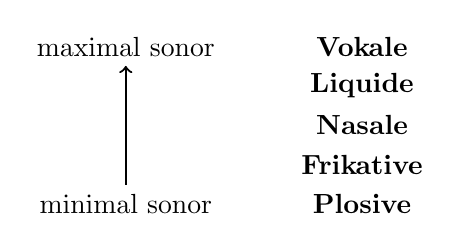
\begin{tikzpicture}
    \node (min)                             {minimal sonor};
    \node (plo) at ([shift={( 3,0)}]   min) {\textbf{Plosive}};
    \node (fri) at ([shift={( 0,0.5)}] plo) {\textbf{Frikative}};
    \node (nas) at ([shift={( 0,0.5)}] fri) {\textbf{Nasale}};
    \node (liq) at ([shift={( 0,0.5)}] nas) {\textbf{Liquide}};
    \node (vok) at ([shift={( 0,0.5)}] liq) {\textbf{Vokale}};
    \node (max) at ([shift={(-3,0)}]   vok) {maximal sonor};
    \draw [->, thick] (min) to (max);
  \end{tikzpicture}
  \caption{Sonoritätshierarchie}
  \label{fig:sonoritaetshierarchie}
\end{figure}

\begin{figure}[!htbp]
  \centering
  \begin{tikzpicture}
    \node (P1) at (0, 0.0) {P};
    \node (F1) at (1, 0.5) {F};
    \node (N1) at (2, 1.0) {N};
    \node (L1) at (3, 1.5) {L};
    \node (V0) at (4, 2.0) {V};
    \node (L2) at (5, 1.5) {L};
    \node (N2) at (6, 1.0) {N};
    \node (F2) at (7, 0.5) {F};
    \node (P2) at (8, 0.0) {P};
    \draw [->] (P1) to (F1);
    \draw [->] (F1) to (N1);
    \draw [->] (N1) to (L1);
    \draw [->] (L1) to (V0);
    \draw [->] (V0) to (L2);
    \draw [->] (L2) to (N2);
    \draw [->] (N2) to (F2);
    \draw [->] (F2) to (P2);
  \end{tikzpicture}
  \caption{Sonorität für die Segmentklassen in der schematischen Silbe}
  \label{fig:sonhier}
\end{figure}

Innerhalb der Silbe gibt es das universelle Bildungsprinzip der \textit{Sonoritätskontur}, welches regelt, dass die Sonorität zum Vokal hin ansteigt und dann wieder abfällt, wie in Abbildung~\ref{fig:sonhier} schematisch dargestellt.\index{Sonorität}
Eine Silbe, die nur aus einem Plosiv und einem Vokal besteht, zeigt einen Sonoritätsanstieg, aber keinen Sonoritätsabfall.
Es gibt also Silben, die nur einen Ausschnitt aus der Sonoritätskontur realisieren (nur Anstieg oder nur Abfall), aber einen Sonoritätsabfall gefolgt von einem Anstieg gibt es innerhalb einzelner Silben im Normalfall nicht.
Definition~\ref{def:sonoritaet} fasst zusammen.

\Definition{Sonorität und Sonoritätskontur}{\label{def:sonoritaet}%
Segmente können auf einer \textit{Sonoritätsskala} eingeordnet werden.
Alle zulässigen Silbenstrukturen stellen einen Anstieg der Sonorität zur Mitte der Silbe und einen Abfall der Sonorität zum Ende der Silbe (oder einen Ausschnitt aus einem solchen Verlauf) dar.
Sie weisen also eine steigende--fallende \textit{Sonoritätskontur} auf.
\index{Sonorität}
}

\begin{exe}
  \ex\label{ex:silbenbau}
  \begin{xlist}
    \ex\label{ex:silbenbau1} \textit{Kuh}\leavevmode
      \SonDiag[2]{{k/\plo/0, u:/\vok/0}}\\[\baselineskip]
    \ex\label{ex:silbenbau1} \textit{nie}\leavevmode
      \SonDiag[2]{{n/\nas/0, i:/\vok/0}}\\[\baselineskip]
    \ex\label{ex:silbenbau1} \textit{Knie}\leavevmode
      \SonDiag[3]{{k/\plo/0, n/\nas/0, i:/\vok/0}}\\[\baselineskip]
    \ex\label{ex:silbenbau1} \textit{droh}\leavevmode
      \SonDiag[3]{{d/\plo/0, K/\liq/0, o:/\vok/0}}\\[\baselineskip]
    \ex\label{ex:silbenbau1} \textit{steh}\leavevmode
      \SonDiag[3]{{S/\fri/2, t/\plo/0, e:/\vok/0}}\\[\baselineskip]
    \ex\label{ex:silbenbau1} \textit{Schnee}\leavevmode
      \SonDiag[3]{{S/\fri/0, n/\nas/0, e:/\vok/0}}\\[\baselineskip]
    \ex\label{ex:silbenbau1} \textit{sprüh}\leavevmode
      \SonDiag[4]{{S/\fri/2, p/\plo/0, K/\liq/0, y:/\vok/0}}\\[\baselineskip]
    \ex\label{ex:silbenbau1} \textit{ab}\leavevmode
      \SonDiag[3]{{P/\plo/0, a/\vok/0, p/\plo/0}}\\[\baselineskip]
    \ex\label{ex:silbenbau1} \textit{an}\leavevmode
      \SonDiag[3]{{P/\plo/0, a/\vok/0, n/\nas/0}}\\[\baselineskip]
    \ex\label{ex:silbenbau1} \textit{acht}\leavevmode
      \SonDiag[4]{{P/\plo/0, a/\vok/0, X/\fri/0, t/\plo/0}}\\[\baselineskip]
    \ex\label{ex:silbenbau1} \textit{Alm}\leavevmode
      \SonDiag[4]{{P/\plo/0, a/\vok/0, l/\liq/0, m/\nas/0}}\\[\baselineskip]
    \ex\label{ex:silbenbau1} \textit{Raps}\leavevmode
      \SonDiag[4]{{K/\fri/0, a/\vok/0, p/\plo/0, s/\fri/2}}\\[\baselineskip]
  \end{xlist}
\end{exe}

In (\ref{ex:silbenbau}) werden zur Illustration einige kurze einsilbige deutsche Wörter in \textit{Sonoritätsdiagrammen} in das Schema eingeordnet.
Das ideale Bild der Sonoritätskontur wird dabei weitgehend bestätigt.
Die einzige Ausnahme ist das Auftreten von den in den Diagrammen eingekreisten \textipa{[S]} vor Plosiven im Anfangsrand (\textit{sprüh}) und [s] nach Plosiven im Endrand (\textit{Raps}).
Da Frikative eine höhere Sonorität haben als Plosive, steigt in diesen Fällen die Sonorität zum Rand hin wieder an.
In Wörtern wie \textit{trittst} setzt sich das Problem sogar noch weiter fort, weil nach dem Anstieg ein weiterer Abfall folgt.
In \textit{Herbsts} folgt nach dem [p] sogar eine Kontur aus Anstieg, Abstieg und erneutem Anstieg, s.\ Abbildung~\ref{fig:sonhierherbsts}.

\begin{figure}[!htbp]
  \centering
  \SonDiag[6]{{h/\fri/0, \t{E@}/\vok/0, p/\plo/0, s/\fri/2, t/\plo/2, s/\fri/2}}
  \caption{Sonorität am Beispiel von \textit{Herbsts}}
  \label{fig:sonhierherbsts}
\end{figure}

Weil solche Sequenzen nicht der Sonoritätsbedingung entsprechen (sowie aus unabhängigen anderen Gründen, die in Abschnitt~\ref{sec:systematikderraender} und Abschnitt~\ref{sec:einsilblerzweisilbler} erläutert werden), betrachten wir die betroffenen Segmente als \textit{extrasilbisch} (außerhalb der normalen Silbenstruktur stehend), vgl.\ Definition~\ref{def:extrasilbisch}.

\Definition{Extrasilbizität}{\label{def:extrasilbisch}\index{Extrasilbizität}%
Die Silbenstruktur kann durch vor dem Anfangsrand oder nach dem Endrand stehende \textit{extrasilbische} Segmente ergänzt werden, die nicht den Bedingungen der Sonoritätskontur unterliegen.}

Es ergibt sich eine erweiterte Silbenstruktur in Abbildung~\ref{fig:silbenstrukturextra}, in der die Sonoritätskontur nur für die Silbe, nicht aber für die mit gestrichelten Linien den Rändern angelehnten extrasilbischen Obstruenten gilt.
In einem Vorgriff auf Abschnitt~\ref{sec:systematikderraender} nehmen wir an, dass maximal zwei Konsonanten (C) im Anfangs- und Endrand stehen können, und dass vor dem Anfangsrand ein extrasilbisches Segment (X) und nach dem Endrand maximal drei extrasilbische Segmente stehen können.

\begin{figure}[!htbp]
  \centering
  \begin{forest}
    [Silbe, calign=last
      [Anfangsrand, sake, calign=child, calign child=2
        [X, edge=dashed][C][C]
      ]
      [Reim, calign=first
        [Kern, sake
          [V]
        ]
        [Endrand, sake, calign=child, calign child=2
          [C][C][X,edge=dashed][X,edge=dashed][X,edge=dashed]
        ]
      ]
    ]
  \end{forest}
  \caption{Schema für die Silbenstruktur mit extrasilbischen Segmenten}
  \label{fig:silbenstrukturextra}
\end{figure}

Außerdem kann die Sonorität auch gleich bleiben, so dass sich \textit{Plateaus} aus zwei Plosiven (\textit{Abt}), zwei Frikativen (\textit{Reichs}) usw.\ bilden.
Abbildung~\ref{fig:sonhiersstrolchst} zeigt die Kontur des Wortes \textit{strolchst} mit extrasilbischem \textipa{[S]} vor dem Anfangsrand und einem Frikativ-Plateau im Endrand.
In Abschnitt~\ref{sec:systematikderraender} werden Plateaus allerdings eliminiert, indem plateaubildendes Material auch als extrasilbisch aufgefasst wird.

\begin{figure}[!htbp]
  \centering
  \SonDiag[8]{{S/\fri/0, t/\plo/0, K/\liq/0, O/\vok/0, l/\liq/0, ç/\fri/0, s/\fri/0, t/\plo/0}}
  \caption{Sonorität am Beispiel von \textit{strolchst}}
  \label{fig:sonhiersstrolchst}
\end{figure}

Was die Sonorität aus phonetisch-artikulatorischer oder perzeptorischer Sicht genau ist, ist eine schwierige Frage.
Stimmhaftigkeit ist ein wichtiger Faktor für eine hohe Sonorität.
Darüber hinaus kann als Faustregel gelten, dass, je enger die durch die Artikulatoren hergestellte Annäherung ist, die Sonorität umso geringer ist.
Dies entspricht dem artikulatorischen Schema des Öffnens und Schließens des Vokaltrakts (Abschnitt~\ref{sec:silben}).

\subsection{Die Systematik der Ränder}

\label{sec:systematikderraender}
\index{Silbe!Rand}

In diesem Abschnitt werden der Anfangsrand und der Endrand im Einsilbler für den Kernwortschatz mit dem Wissen um die Sonoritätshierarchie abschließend beschrieben.
Die Systematisierung des Anfangsrands wird dadurch erreicht, dass \textipa{[S]} in Anfangsrändern mit scheinbar zwei oder drei Segmenten eliminiert wird.%
\footnote{Typenseltene Wörter wie \textit{Skat} enthalten [s] statt \textipa{[S]}.
Wir zählen sie nicht zum Kern.}
In Abschnitt~\ref{sec:sonoritaet} wurde festgestellt, dass \textipa{[S]} vor Plosiven (\textit{Sprung}, \textit{Stuhl}) die Sonoritätshierarchie verletzt.
Vor Frikativen (\textit{Schwung}) entsteht ein Sonoritätsplateau.
Lediglich in mehrsegmentalen Anfangsrändern mit einem Nasal oder Liquid an zweiter Stelle (\textit{Schmal}, \textit{Schrank}, \textit{Schlund}) verhält sich \textipa{[S]} theoretisch konform zur Sonoritätshierarchie.
Zudem sind die einzigen Anfangsränder mit drei Segmenten solche, bei denen das erste Segment \textipa{[S]} ist.
Das Segment \textipa{[S]} verhält sich im Silbenbau offensichtlich besonders, und es wurde mit Definition~\ref{def:extrasilbisch} aus der eigentlichen Silbe in einen erweiterten Bereich verschoben, in dem die Sonoritätskontur nicht eingehalten werden muss.
Es ist \textit{extrasilbisch}.

\begin{figure}[!htbp]
  \centering
  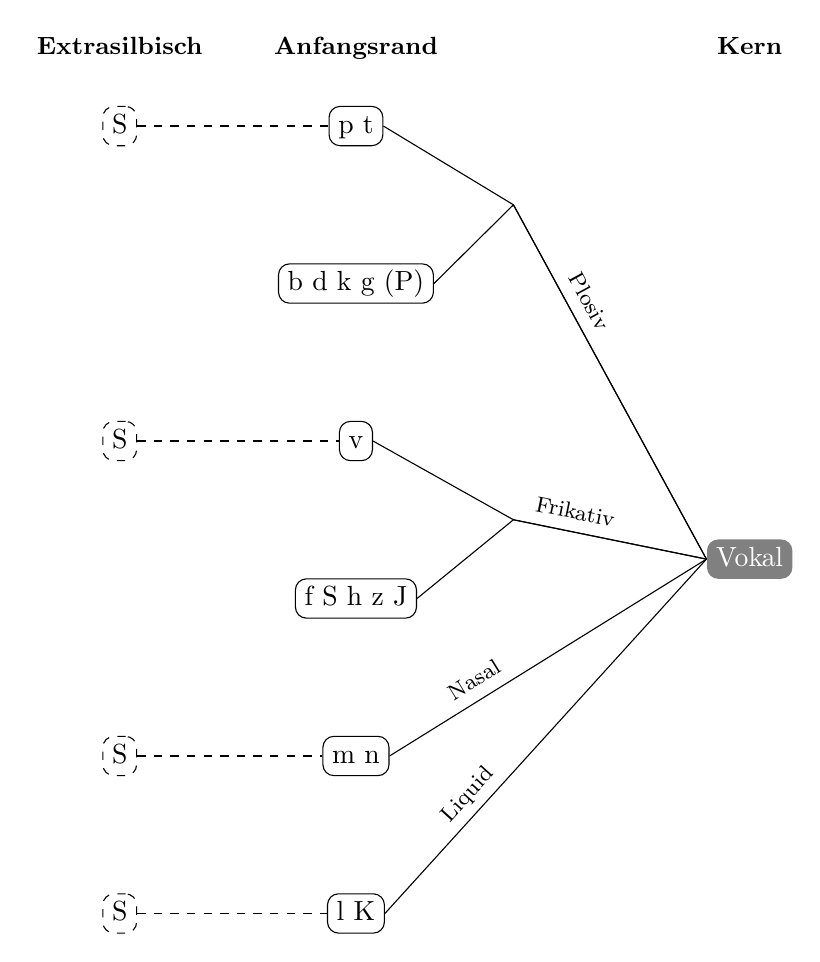
\begin{tikzpicture}[text height=1.5ex, text depth=.25ex, text centered]
    \tikzset{%
      segm/.style={fill=white, draw, rounded corners, execute at begin node=\tipaencoding},
      extrasyl/.style={segm, dashed}
      }
    \node at (0, 12) {\textbf{\small Extrasilbisch}};
    \node at (3, 12) {\textbf{\small Anfangsrand}};
    \node at (8, 12) {\textbf{\small Kern}};

    \node [fill=gray, rounded corners] (Xvok) at (8, 5.5) {\textcolor{white}{Vokal}};

    \node [segm] (Xplu) at (3,11) {p t};
    \node [extrasyl] (XSplu) at (0,11) {S};
    \draw [dashed] (XSplu) to (Xplu);
    \node [segm] (Xplv) at (3,9) {b d k g (P)};
    \draw (Xvok.west) -- node [pos=0.7, above, sloped] {\footnotesize Plosiv} (5, 10) -- (Xplu.east);
    \draw (Xvok.west) -- (5, 10) -- (Xplv.east);

    \node [segm] (Xvov) at (3,7) {v};
    \node [extrasyl] (XSvov) at (0,7) {S};
    \draw [dashed] (XSvov) to (Xvov);
    \node [segm] (Xfri) at (3,5) {f S h z J};
    \draw (Xvok.west) -- node [pos=0.7, above, sloped] {\footnotesize Frikativ} (5, 6) -- (Xvov.east);
    \draw (Xvok.west) -- (5, 6) -- (Xfri.east);

    \node [segm] (Xnas) at (3,3) {m n};
    \node [extrasyl] (XSnas) at (0,3) {S};
    \draw [dashed] (XSnas) to (Xnas);
    \node [segm] (Xliq) at (3,1) {l K};
    \node [extrasyl] (XSliq) at (0,1) {S};
    \draw [dashed] (XSliq) to (Xliq);
    \draw (Xvok.west) to node [pos=0.7, above, sloped] {\footnotesize Nasal} (Xnas.east);
    \draw (Xvok.west) to node [pos=0.7, above, sloped] {\footnotesize Liquid} (Xliq.east);
  \end{tikzpicture}
  \caption{Struktur des simplexen Anfangsrands}
  \label{fig:anfangsrandsimplex}
\end{figure}

Die maximale Komplexität des Anfangsrands besteht also in zwei Segmenten:\index{Silbe!Anfangsrand!komplex}
Der Anfangsrand ist maximal \textit{duplex}.
Scheinbare Fälle von drei Segmenten im Anfangsrand (\textipa{[SpK]}, \textipa{[StK]} und evtl.\ \textipa{[Spl]}) im Anfangsrand bestehen aus zwei Segmenten mit extrasilbischem \textipa{[S]}.
Wenn man \textipa{[S]} diesen Sonderstatus zuweist, dampft die Beschreibung der Besetzungsmöglichkeiten des simplexen Anfangsrands auf Abbildung~\ref{fig:anfangsrandsimplex} und die des duplexen Anfangsrands auf Abbildung~\ref{fig:anfangsrandduplex} ein.
Die Abbildungen sind von rechts nach links zu lesen, und sie bilden die \textit{Besetzungsmöglichkeiten} des Anfangsrands ab.
Für jede mögliche Besetzung des Anfangsrands gibt es genau einen Weg durch die Äste des Diagramms.
Man beginnt mit dem Vokal im Kern.
Die von dort nach links weisenden Äste zeigen Besetzungsmöglichkeiten für das erste Segment im Anfangsrand links vom Vokal.
Von diesen weisen ggf.\ weitere Äste nach links, die die Möglichkeiten für weiter links stehende Segmente anzeigen, und zwar abhängig von dem bereits eingeschlagenen Weg.
Die in Gruppen angeordneten Segmente stellen jeweils verschiedene Möglichkeiten der Besetzung dar.
In Abbildung~\ref{fig:anfangsrandsimplex} kann man vor dem Vokal zum Beispiel einen Plosiv einsetzen (oberer Ast).
Es kommen \textipa{[p]} oder \textipa{[t]} infrage (obere Verästelung des obersten Asts), vor dem noch ein \textipa{[S]} stehen kann.
Vor \textipa{[b]}, \textipa{[d]}, \textipa{[k]} und \textipa{[g]} (untere Verästelung des oberen Asts) kann allerdings kein \textipa{[S]} stehen.
Der Glottalplosiv \textipa{[P]} ist eingeklammert, um seinen Sonderstatus als nicht zugrundeliegendes Segment zu markieren.


Es wird sofort deutlich, dass die Kombinationsmöglichkeiten sehr stark auf die Verbindung von Plosiven oder den labiodentalen Frikativen [f] und [v] mit folgendem Liquid eingeschränkt sind.
Zwischen den beiden Liquiden an zweiter Stelle gibt es im Wesentlichen zwei minimale Unterschiede.
Einerseits kommen die Kombinationen \textipa{[tK]} (\textit{Trog}) und \textipa{[dK]} (\textit{Druck}), nicht aber die Kombinationen \textipa{[tl]} und \textipa{[dl]} vor.%
\footnote{Diese Einschränkung kann man damit erklären, dass \textipa{[l]} den gleichen Artikulationsort wie \textipa{[t]} und \textipa{[d]} hat, und dass die Segmente dadurch zu ähnlich sind, um im Anfangsrand zusammen vorzukommen.
Eine \textit{Erklärung} im Sinne einer kausalen Beziehung wird daraus allerdings ohne erheblichen argumentativen Mehraufwand und Zusatzannahmen nicht, zumal an anderer Stelle (bei Assimilationen) sogar eine Angleichung von Artikulationsorten gefordert wird.}
Andererseits ist \textipa{[vK]} möglich (\textit{wringen}), aber (im Kern des Systems) nicht \textipa{[vl]} (vgl.\ aber peripher \textit{Vladimir} usw.).
In Satz~\ref{satz:anfangsrand} wird die Struktur des Anfangsrands kompakt beschrieben.


\Satz{Anfangsrand}{\label{satz:anfangsrand}%
Der Anfangsrand ist maximal duplex.
Die präferierte Besetzung des duplexen Anfangsrands ist die aus einem inneren Liquid und einem äußeren Obstruenten.
Extrasilbisch tritt ggf.\ \textipa{[S]} vor den Anfangsrand.\index{Silbe!Anfangsrand!komplex}}

\begin{figure}[!htbp]
  \centering
  \resizebox{!}{0.95\textheight}{
  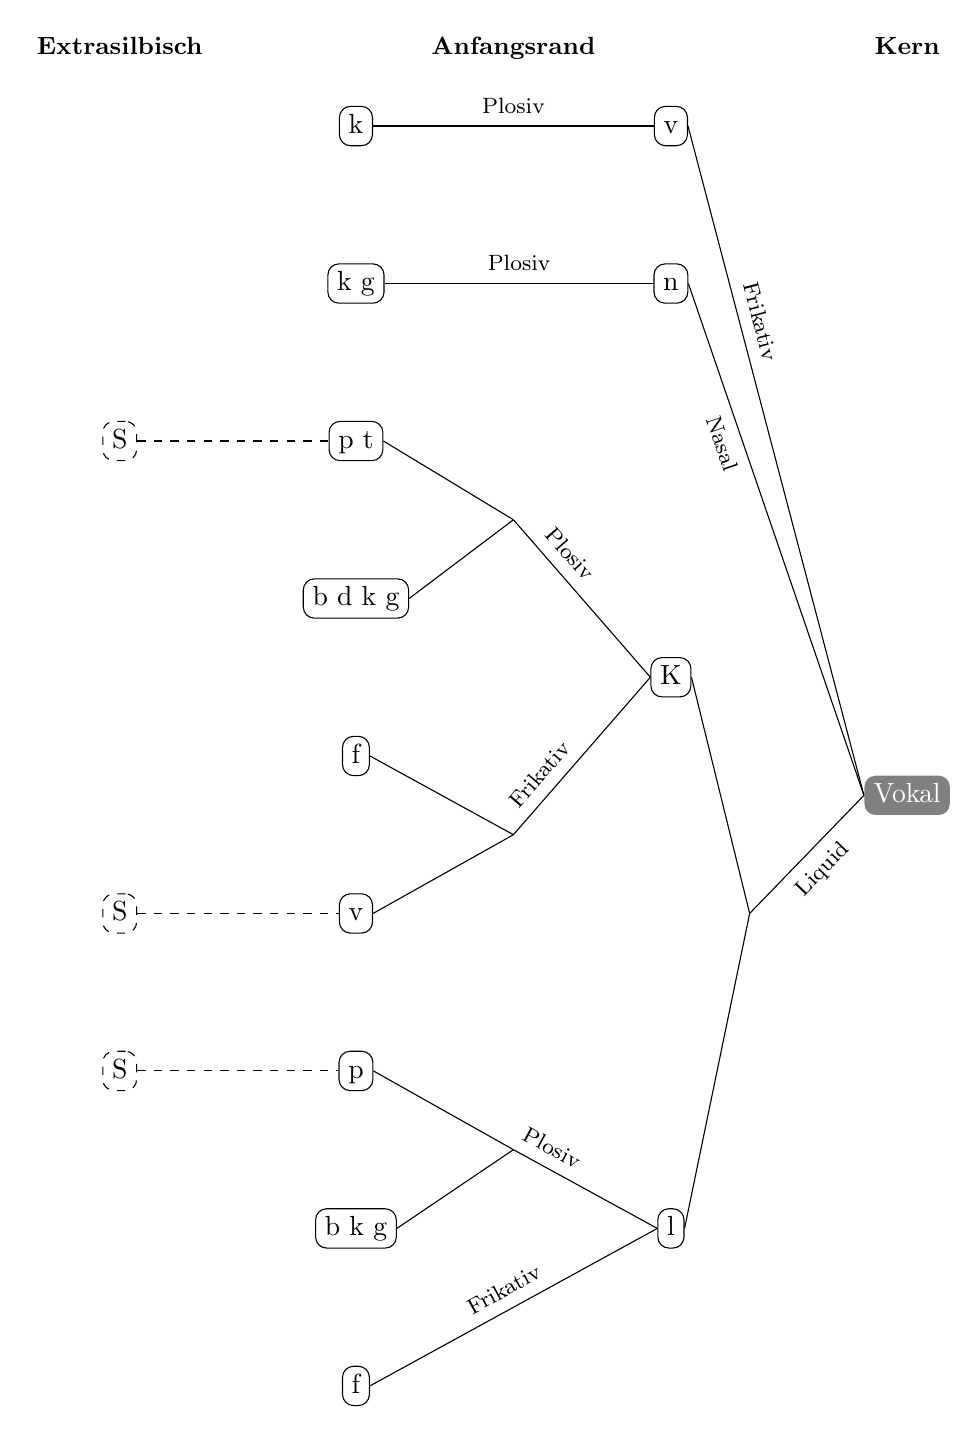
\begin{tikzpicture}[text height=1.5ex, text depth=.25ex, text centered]
    \tikzset{%
      segm/.style={fill=white, draw, rounded corners, execute at begin node=\tipaencoding},
      extrasyl/.style={segm, dashed}
      }
    \node at (0, 18) {\textbf{\small Extrasilbisch}};
    \node at (5, 18) {\textbf{\small Anfangsrand}};
    \node at (10, 18) {\textbf{\small Kern}};

    \node [fill=gray, rounded corners] (Yvok) at (10, 8.5) {\textcolor{white}{Vokal}};

    \node [segm] (Yk) at (3,17) {k};
    \node [segm] (Yv) at (7,17) {v};
    \draw (Yk.east) -- node [pos=0.5, above] {\footnotesize Plosiv} (Yv.west);
    \draw (Yvok.west) -- node [pos=0.7, above, sloped] {\footnotesize Frikativ} (Yv.east);

    \node [segm] (Ykg) at (3,15) {k g};
    \node [segm] (Yn) at (7,15) {n};
    \draw (Ykg.east) -- node [pos=0.5, above] {\footnotesize Plosiv} (Yn.west);
    \draw (Yvok.west) -- node [pos=0.7, below, sloped] {\footnotesize Nasal} (Yn.east);

    \node [segm] (Ypt) at (3,13) {p t};
    \node [extrasyl] (YSpt) at (0,13) {S};
    \draw [dashed] (YSpt) to (Ypt);
    \node [segm] (Ybdkg) at (3,11) {b d k g};
    \node [segm] (Yf) at (3,9) {f};
    \node [segm] (Yv1) at (3,7) {v};
    \node [extrasyl] (YSv1) at (0,7) {S};
    \draw [dashed] (YSv1) to (Yv1);

    \node [segm] (YR) at (7,10) {K};
    \draw (Ypt.east) -- (5,12);
    \draw (Ybdkg.east) -- (5,12);
    \draw (5,12) -- node [pos=0.3, above, sloped] {\footnotesize Plosiv} (YR.west);
    \draw (Yf.east) -- (5,8);
    \draw (Yv1.east) -- (5,8);
    \draw (5,8) -- node [pos=0.3, above, sloped] {\footnotesize Frikativ} (YR.west);

    \node [segm] (Yp) at (3,5) {p};
    \node [extrasyl] (YSp) at (0,5) {S};
    \draw [dashed] (YSp) to (Yp);
    \node [segm] (Ybkg) at (3,3) {b k g};
    \node [segm] (Yff) at (3,1) {f};

    \node [segm] (Yl) at (7,3) {l};
    \draw (Yp.east) -- (5,4);
    \draw (Ybkg.east) -- (5,4);
    \draw (5,4) -- node [pos=0.2, above, sloped] {\footnotesize Plosiv} (Yl.west);
    \draw (Yff.east) -- node [pos=0.5, above, sloped] {\footnotesize Frikativ} (Yl.west);

    \draw (YR.east) -- (8,7);
    \draw (Yl.east) -- (8,7);
    \draw (8,7) -- node [pos=0.5, below, sloped] {\footnotesize Liquid} (Yvok.west);

  \end{tikzpicture}}
  \caption{Struktur des duplexen Anfangsrands}
  \label{fig:anfangsrandduplex}
\end{figure}

Bei der deskriptiven Sichtung in Abschnitt~\ref{sec:endrandimeinsilbler} schien der Endrand drei oder mehr Segmente enthalten zu können.\index{Silbe!Endrand!komplex}
Wir beschreiben jetzt zunächst den duplexen Endrand und versuchen, davon ausgehend weiter zu systematisieren.
Alle Kombinationen, die eine Verletzung der Sonoritätskontur darstellen würden, werden dabei gleich ausgeschlossen.
Außerdem wird \textipa{[N]} als zugrundeliegendes Segment aus dem System eliminiert (mehr dazu weiter unten).
Es ergibt sich Abbildung~\ref{fig:endranduplex}, die den duplexen Endrand ohne extrasilbisches Material abbildet.

\begin{figure}[!htbp]
  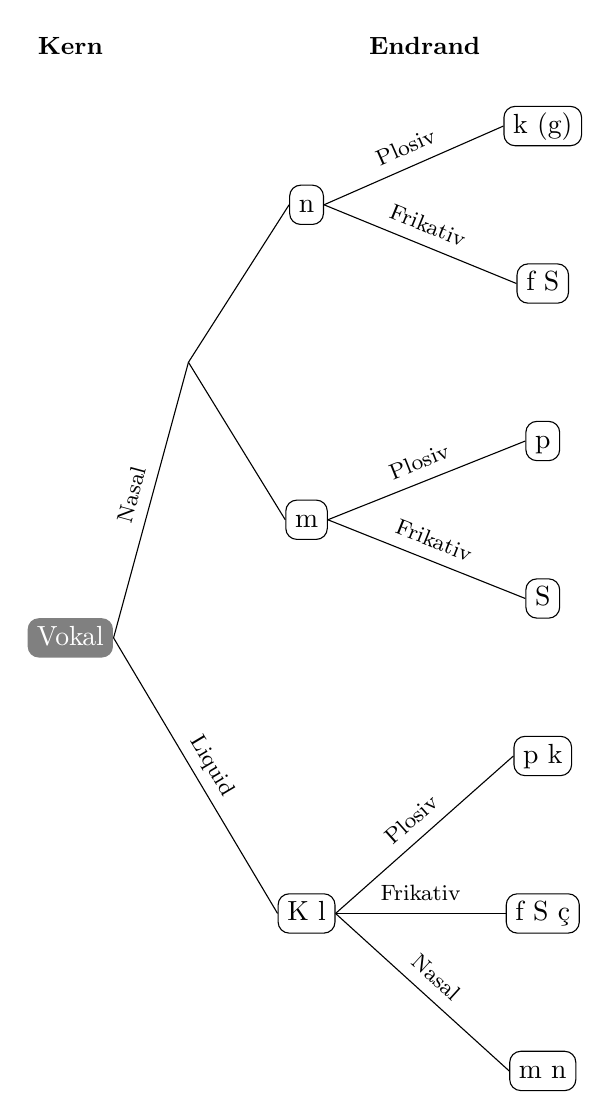
\begin{tikzpicture}[text height=1.5ex, text depth=.25ex, text centered]
    \tikzset{%
      segm/.style={fill=white, draw, rounded corners, execute at begin node=\tipaencoding},
      extrasyl/.style={segm, dashed}
      }
    \node at (0, 14) {\textbf{\small Kern}};
    \node at (4.5, 14) {\textbf{\small Endrand}};

    \node [fill=gray, rounded corners] (Zvok) at (0, 6.5) {\textcolor{white}{Vokal}};

     \node [segm] (Zkg) at (6,13) {k (g)};
     \node [segm] (ZfS) at (6,11) {f S};

     \node [segm] (Zn) at (3,12) {n};
     \draw (Zn.east) -- node [pos=0.5, above, sloped] {\footnotesize Plosiv} (Zkg.west);
     \draw (Zn.east) -- node [pos=0.5, above, sloped] {\footnotesize Frikativ} (ZfS.west);

     \node [segm] (Zp) at (6,9) {p};
     \node [segm] (ZS) at (6,7) {S};

     \node [segm] (Zm) at (3,8) {m};
     \draw (Zm.east) -- node [pos=0.5, above, sloped] {\footnotesize Plosiv} (Zp.west);
     \draw (Zm.east) -- node [pos=0.5, above, sloped] {\footnotesize Frikativ} (ZS.west);

     \draw (Zvok.east) --  node [pos=0.5, above, sloped] {\footnotesize Nasal} (1.5,10);
     \draw (1.5,10) -- (Zn.west);
     \draw (1.5,10) -- (Zm.west);

     \node [segm] (Zpk) at (6,5) {p k};
     \node [segm] (ZfSc) at (6,3) {f S ç};
     \node [segm] (Zmn) at (6,1) {m n};

     \node [segm] (ZRl) at (3,3) {K l};
     \draw (ZRl.east) -- node [pos=0.5, above, sloped] {\footnotesize Plosiv} (Zpk.west);
     \draw (ZRl.east) -- node [pos=0.5, above, sloped] {\footnotesize Frikativ} (ZfSc.west);
     \draw (ZRl.east) -- node [pos=0.5, above, sloped] {\footnotesize Nasal} (Zmn.west);

     \draw (Zvok.east) -- node [pos=0.5, above, sloped] {\footnotesize Liquid} (ZRl.west);

  \end{tikzpicture}
  \caption{Struktur des duplexen Endrands}
  \label{fig:endranduplex}
\end{figure}

Das Diagramm in Abbildung~\ref{fig:endranduplex} beschreibt nicht alle Endränder, die rein oberflächlich gesehen duplex sind.
Zunächst müssen Wörter wie in (\ref{ex:phol7528}) anders erklärt werden, wenn Abbildung~\ref{fig:endranduplex} allgemein gelten soll.

\begin{exe}
  \ex \label{ex:phol7528}
  \begin{xlist}
    \ex{\label{ex:phol7528a} Schnaps, Huts, zwecks}
    \ex{\label{ex:phol7528b} Abt, nackt}
    \ex{\label{ex:phol7528d} Laufs, Reichs}
  \end{xlist}
\end{exe}

Die Wörter in (\ref{ex:phol7528a}) enthalten ein [s], das die Sonoritätskontur verletzt.
Wie schon im Anfangsrand behandeln wir es als extrasilbisch.
Das [t] in (\ref{ex:phol7528b}) bildet mit den vorangehenden Plosiven ein Sonoritätsplateau.
In Fällen wie \textit{trittst} muss nun [t] außerdem ohnehin extrasilbisch sein, wenn das vorangehende [s] bereits extrasilbisch ist.
Zudem sind sowohl [t] als auch [s] alveolare Obstruenten, und bilden damit eine (wenn auch kleine) Klasse.
Wir nehmen daher an, dass Segmente aus genau dieser Klasse der alveolaren Obstruenten extrasilbisch an den Endrand treten können.
Das ein Plateau bildende [s] in (\ref{ex:phol7528d}) kann nun ebenfalls extrasilbisch interpretiert werden.
Damit müssen (wie im Anfangsrand) auch im Endrand keine Frikativ-Plateaus angenommen werden.
Wie noch demonstriert werden wird, eliminieren wir durch die Annahme von extrasilbischem [t] und [s] Endränder mit mehr als zwei Segmenten vollständig aus dem System.
Das System wird so simpel, wie es in Abbildung~\ref{fig:endranduplex} aussieht.
Die Beziehung von zugrundeliegender Form und phonetischer Oberfläche wird in (\ref{ex:phol0800009003}) gezeigt, wo extrasilbische Segmente mit + abgetrennt sind.

\begin{exe}
  \ex \label{ex:phol0800009003}
  \begin{xlist}
    \ex{\label{ex:phol0800009003a} /\textipa{huts}/ $\Rightarrow$ \textipa{[hu:t+s]} (\textit{Huts})}
    \ex{\label{ex:phol0800009003b} /\textipa{Sn\u{a}ps}/ $\Rightarrow$ \textipa{[S+nap+s]} (\textit{Schnaps})}
    \ex{\label{ex:phol0800009003c} /\textipa{\t{ts}v\u{E}ks}/ $\Rightarrow$ \textipa{[\t{ts}vEk+s]} (\textit{zwecks})}
    \ex{\label{ex:phol0800009003d} /\textipa{\u{a}pt}/ $\Rightarrow$ \textipa{[Pap+t]} (\textit{Abt})}
    \ex{\label{ex:phol0800009003e} /\textipa{n\u{a}kt}/ $\Rightarrow$ \textipa{[nak+t]} (\textit{nackt})}
    \ex{\label{ex:phol0800009003f} /\textipa{l\t{aO}fs}/ $\Rightarrow$ \textipa{[l\t{aO}f+s]} (\textit{Laufs})}
  \end{xlist}
\end{exe}

Die Kombinationen aus Frikativ und [t] können auch generell als simplexe Endränder mit extrasilbischem [t] aufgefasst werden.
Deswegen gibt es in Abbildung~\ref{fig:endranduplex} gar keinen Ast für Frikative nach dem Vokal.
Dafür, dass es sich dabei nicht etwa um einen phonologischen Taschenspielertrick handelt, wird in Abschnitt~\ref{sec:einsilblerzweisilbler} weiter argumentiert.
Die sich ergebenden Formen zeigt (\ref{ex:phol08000090035}).

\begin{exe}
  \ex \label{ex:phol08000090035}
  \begin{xlist}
    \ex{\label{ex:phol08000090035a} /\textipa{Kuft}/ $\Rightarrow$ \textipa{[Ku:f+t]} (\textit{ruft})}
    \ex{\label{ex:phol08000090035b} /\textipa{\u{a}\c{c}t}/ $\Rightarrow$ \textipa{[PaX+t]} (\textit{Acht})}
    \ex{\label{ex:phol08000090035c} /\textipa{l\u{E}st}/ $\Rightarrow$ \textipa{[lEs+t]} (\textit{lässt})}
  \end{xlist}
\end{exe}

Bei den Endrändern mit Nasal als erstes Segment sind vor allem zwei Merkwürdigkeiten in Abbildung~\ref{fig:endranduplex} zu begründen.
Einerseits fehlt \textipa{[N]} vollständig, andererseits kommt nach [n] angeblich ein [g] vor, wobei dieses in Abbildung~\ref{fig:endranduplex} eingeklammert ist.
Im Endrand sollte ja eigentlich wegen der Auslautverhärtung kein stimmhafter Plosiv vorkommen können.

Mögliche zweisegmentale Endränder mit velarem Nasal \textipa{[N]} an der phonetischen Oberfläche findet man in Wörtern mit nachfolgendem velaren Plosiv wie \textit{krank} \textipa{[kKaNk]}.
Es fällt insgesamt auf, dass zwar [t] mit allen Nasalen kombiniert werden kann (\textit{klemmt}, \textit{rennt}, \textit{hängt}), [p] aber nur mit [m] (\textit{Lump}) und [k] nur mit \textipa{[N]} (\textit{krank}).
Es liegt der Verdacht nahe, dass hier eigentlich nur homorgane (am selben Ort artikulierte) Sequenzen aus Nasal und Plosiv vorkommen können.
Es kann eventuell sogar von /\textipa{kKank}/ \phopro \textipa{[kKaNk]} und /\textipa{lUnp}/ \phopro \textipa{[lUmp]} ausgegangen werden.
Ein [t] nach [m] oder \textipa{[N]} wie in \textit{klemmt} oder \textit{hängt} ist dann als extrasilbisch zu analysieren.

Was ist aber mit dem einfachen \textipa{[N]} wie in \textit{Gang}?
Hier folgt dem velaren Nasal kein velarer Plosiv, an den er seinen Artikulationsort anpassen könnte.
Wir führen \textipa{[N]} daher auf eine zugrundeliegende Kombination /ng/ zurück.
Der Nasal /n/ assimiliert an /g/ zu \textipa{[N]}, und das /g/ wird nicht artikuliert.
Phonologisch und aus Sicht der Silbifizierung haben wir es \zB in /gang/ also mit einem duplexen Endrand zu tun, phonetisch mit einem simplexen.
Weil es phonetisch (in der betreffenden Position) niemals auftritt, ist \textipa{[g]} in Abbildung~\ref{fig:endranduplex} eingeklammert.
Die Analyse von \textipa{[N]} als /ng/ eliminiert \textipa{[N]} als zugrundeliegendes Segment, weswegen es konsequent in [~] statt in /~/ geschrieben werden sollte.
Für diese Reduktion des Systems wird in Abschnitt~\ref{sec:einsilblerzweisilbler} weiter argumentiert, da sich \textipa{[N]} als phonetisches Korrelat zu /ng/ im Endrand auch in anderer Hinsicht wie zwei Segmente verhält.

Die Beziehung zugrundeliegender Formen und ihrer phonetischen Realisierungen in einigen kritischen Formen illustriert (\ref{ex:phol0800009004}).

\begin{exe}
  \ex \label{ex:phol0800009004}
  \begin{xlist}
    \ex{\label{ex:phol0800009004a} /\textipa{g\u{a}ng}/ $\Rightarrow$ \textipa{[gaN]} (\textit{Gang})}
    \ex{\label{ex:phol0800009004b} /\textipa{l\u{E}ngs}/ $\Rightarrow$ \textipa{[lEN+s]} (\textit{längs})}
    \ex{\label{ex:phol0800009004c} /\textipa{h\u{E}ngt}/ $\Rightarrow$ \textipa{[hEN+t]} (\textit{hängt})}
    \ex{\label{ex:phol0800009004d} /\textipa{kr\u{a}nk}/ $\Rightarrow$ \textipa{[kraNk]} (\textit{krank})}
    \ex{\label{ex:phol0800009004e} /\textipa{kl\u{E}mt}/ $\Rightarrow$ \textipa{[klEm+t]} (\textit{klemmt})}
    \ex{\label{ex:phol0800009004f} /\textipa{bUnt}/ $\Rightarrow$ \textipa{[bUnt]} (\textit{bunt})}
  \end{xlist}
\end{exe}

Es fällt außerdem auf, dass häufig -- wenn auch nicht immer -- extrasilbisches Material (konkret [t], [s] oder [st]) zu sogenannten \textit{Flexionsendungen} gehört, also nicht zum sogenannten \textit{Wortstamm} (vgl.\ Abschnitt~\ref{sec:stamm}).\index{Extrasilbizität!und Flexionssuffixe}
Mit der Grenze zwischen echtem Endrand und extrasilbischem Material fällt also oft auch die Grenze zwischen Stamm und Flexionsendung zusammen, \zB \textit{lebst} \textipa{[le:p+st]}, \textit{glaubt} \textipa{[gl\t{aO}p+t]} oder \textit{Stifts} \textipa{[StIft+s]}.

Zusammenfassend kann man -- wie schon in umgekehrter Reihenfolge beim Anfangsrand -- festhalten, dass der prototypische duplexe Endrand aus einem innerem Liquid und einem äußerem Obstruenten besteht.
Dem Endrand nachfolgende [s] und [t] sind als extrasilbisch zu werten.
In (\ref{ex:phol0800009005}) finden sich weitere Beispiele, wobei (\ref{ex:phol0800009005a}) als Referenzbeispiel ohne extrasilbische Konsonanten angegeben wird.

\begin{exe}
  \ex \label{ex:phol0800009005}
  \begin{xlist}
    \ex{\label{ex:phol0800009005a} /\textipa{kOKb}/ $\Rightarrow$ \textipa{[k\t{O@}p]} (\textit{Korb})}
    \ex{\label{ex:phol0800009005b} /\textipa{vIKbst}/ $\Rightarrow$ \textipa{[v\t{I@}p+st]} (\textit{wirbst})}
    \ex{\label{ex:phol0800009005c} /\textipa{fUK\c{c}t}/ $\Rightarrow$ \textipa{[f\t{U@}\c{c}+t]} (\textit{Furcht})}
    \ex{\label{ex:phol0800009005d} /\textipa{f\u{E}lSst}/ $\Rightarrow$ \textipa{[fElS+st]} (\textit{fälschst})}
  \end{xlist}
\end{exe}

Vor einer weiteren Vertiefung der strukturellen Zusammenhänge, die in Abschnitt~\ref{sec:einsilblerzweisilbler} erfolgen wird, halten wir in Satz~\ref{satz:endrandbesetzung} fest, dass die Besetzungspräferenzen im Endrand nahezu spiegelbildlich dieselben wie im Anfangsrand sind.%
\footnote{Als echte Auslassung im Interesse einer eleganteren Darstellung wurde in Abbildung~\ref{fig:endranduplex} die Besetzung des Endrands aus zugrundeliegendem /\textipa{Kl}/ wie in \textit{Kerl} unterschlagen.
Diese ist im Anfangsrand weder in dieser Reihenfolge noch spiegelbildlich zulässig.
Es drängt sich der Gedanke auf, dass diese Besetzung deshalb möglich ist, weil hier /\textipa{K}/ als zweites Element in einem sekundären Diphthong artikuliert wird (s.\ Abschnitt~\ref{sec:orthographischesr}), also /\textipa{k\u{E}Kl}/ \phopro \textipa{[k\t{E@}l]}.
Im Grunde stellen wir damit die Frage, ob das zweite Element von sekundären und ggf. auch primären Diphthongen eine Position im Kern oder im Endrand besetzt.
Eine zufriedenstellende Analyse solcher komplexer Bedingungen ist meiner Ansicht nur in formal ausgearbeiteten Theorien möglich.}

\Satz{Endrand}{\label{satz:endrandbesetzung}\index{Silbe!Endrand!komplex}
Der Endrand ist maximal duplex.
Die präferierte Besetzung des duplexen Endrands ist die aus einem inneren Liquid und einem äußeren Obstruenten.
Bereits weniger präferiert wird er mit einem Nasal und einem homorganen Plosiv besetzt.
Extrasilbisch treten die alveolaren Obstruenten [s] und [t] hinter den Endrand.}


\subsection{Einsilbler und Zweisilbler}

\label{sec:einsilblerzweisilbler}

\index{Silbe!Silbifizierung}
\index{Einsilbler}
\index{Zweisilbler}

Nach den Silben ist die nächstgrößere Einheit der phonologischen Strukturbildung das \textit{phonologische Wort}.
Der Grund, warum man eine solche Einheit annehmen möchte, ist, dass es phonologische Regularitäten gibt, die sich nicht nur mit Bezug auf Segmente und einzelne Silben beschreiben lassen, vgl.\ Definition~\ref{def:phonwort}.%
\footnote{Es müsste eigentlich der \textit{Fuß} als nächstgrößere Einheit nach der Silbe definiert werden.
Wir gehen nur in Abschnitt~\ref{sec:wortakzentimdeutschen} kurz auf den Fuß ein und wählen daher hier eine vereinfachte Darstellung.}

\Definition{Phonologisches Wort}{\label{def:phonwort}%
Ein \textit{phonologisches Wort} ist die kleinste phonologische Struktur, die Silben als Konstituenten hat, und bezüglich derer eigene Regularitäten feststellbar sind.
\index{Wort!phonologisch}
}

Definition~\ref{def:phonwort} kommt sehr formal daher.
Denken wir aber an den Grammatikbegriff aus Definition~\ref{def:grammatik} (S.~\pageref{def:grammatik}), dann ist die Einschränkung \textit{bezüglich derer eigene Regularitäten feststellbar sind} aber ausgesprochen instruktiv.
Wenn es nämlich phonologische Regularitäten gibt, die sich nicht effektiv und angemessen mit Bezug auf Segmente und Silben beschreiben lassen, müssen wir eine andere, größere Einheit annehmen, bezüglich derer wir sie beschreiben können.
Eine solche Regularität wird in (\ref{ex:phol0815}) illustriert und im Rest dieses Abschnitts analysiert.
Im Sinn einer übersichtlichen Darstellung beschränken wir uns hier auf die Vokale \textipa{[I]} und \textipa{[i]}, aber die Regularitäten gelten für alle Paare von ungespannten und gespannten Vokalen.


\begin{exe}
  \ex\label{ex:phol0815}
  \begin{xlist}
    \ex{\label{ex:phol0815a} Knie \textipa{[kni:]}}
    \ex{\label{ex:phol0815b} *\textipa{[knI]}}
    \ex{\label{ex:phol0815c} schief \textipa{[Si:f]}}
    \ex{\label{ex:phol0815d} Schiff \textipa{[SIf]}}
    \ex{\label{ex:phol0815e} wink \textipa{[vINk]}}
    \ex{\label{ex:phol0815f} *\textipa{[vi:Nk]}}
    \ex{\label{ex:phol0815g} Mie.te \textipa{[mi:.t@]}}
    \ex{\label{ex:phol0815h} Mi.tte \textipa{[mI.t@]}}
    \ex{\label{ex:phol0815i} liebte \textipa{[li:p.t@]}}
    \ex{\label{ex:phol0815j} winkte \textipa{[vINk.t@]}}
    \ex{\label{ex:phol0815k} *\textipa{[vi:Nk.t@]}}
  \end{xlist}
\end{exe}

Die Wörter in (\ref{ex:phol0815}) sind entweder Einsilbler, oder sie sind Zweisilbler, die aus einer Silbe mit einem betonten gespannten (langen) oder einem betonten ungespannten (kurzen) Vokal sowie einer Schwa-Silbe bestehen.
Dieses Muster der Silbenfolge ist charakteristisch für das Deutsche (s.\ auch Abschnitt~\ref{sec:wortakzentimdeutschen}).
Uns interessiert jetzt hier vor allem die Silbenstruktur in der jeweils ersten Silbe.
Als zweite Silbe kommen hier nur Schwa-Silben vor, die von den zu beschreibenden Regularitäten als einzige nicht betroffen sind, weil sie prinzipiell nicht betonbar sind.
Es geht jetzt also um prinzipiell \textit{betonbare Silbentypen}.
Zunächst wird der Sprachgebrauch von der \textit{offenen} und der \textit{geschlossenen Silbe} in Definition~\ref{def:offengeschlossen} eingeführt, der die weitere Argumentation vereinfacht.


\Definition{Offene und geschlossene Silben}{\label{def:offengeschlossen}%
Silben mit gefülltem Endrand sind \textit{geschlossene Silben}, Silben mit leerem Endrand sind \textit{offene Silben}.
\index{Silbe!offen}
\index{Silbe!geschlossen}
}


Zunächst müssen also Einsilbler mit ungespanntem Vokal geschlossen sein, \zB \textit{Schiff} im Vergleich mit unmöglichen Wörtern wie *\textipa{[knI]} oder auch *\textipa{[tO]} usw.
Das gilt auch für die letzte Silbe in Mehrsilblern, also *\textipa{[kUn.dI]} oder *\textipa{[tu:.bO]} usw.
Die einzige Ausnahme bilden Schwa-Silben, die offen als Endsilbe im Mehrsilbler vorkommen können, vgl.\ \textit{Mitte} \textipa{[mi.t@]}.
Wenn der Vokal gespannt ist, kann die Silbe offen sein wie in \textit{Knie}, muss sie aber nicht, vgl.\ \textit{schief}.
Wenn der Endrand des Einsilblers duplex ist wie in \textit{wink}, sind gespannte Vokale nicht möglich, wie das strukturell unmögliche Wort *\textipa{[vi:Nk]} zeigt.
Die Bedingung, dass Silben mit ungespanntem Vokal einen gefüllten Endrand haben müssen, gilt im Zweisilbler nicht, wie \textit{Mi.tte} demonstriert.
Ansonsten gilt aber trotzdem, dass Silben nicht einen gespannten Vokal im Kern und gleichzeitig einen komplex besetzten Endrand haben können, s.\ *\textipa{[vi:Nk.t@]} verglichen mit \textit{winkte} \textipa{[vINk.t@]}.
Diese Verhältnisse lassen sich mit Bezug auf eine Einheit für das \textit{Gewicht} von Silben gut beschreiben, die \textit{More} (Definition~\ref{def:more}).


\Definition{Silbengewicht und More}{\label{def:more}%
Das \textit{Gewicht einer Silbe} ist die Anzahl der Moren im Reim der Silbe.
Ein ungespannter Vokal im Kern und ein einzelner Konsonant im Endrand zählen jeweils als eine \textit{More}, gespannte Vokale und Diphthonge als zwei.
Extrasilbische Segmente tragen nicht zur Morenzahl bei.
\index{Silbe!Gewicht}
\index{More}
\index{Vokal!Gespanntheit}
}

Um die Verteilung der gespannten und ungespannten Vokale und damit die Vokallängen in offenen und geschlossenen Silben sowohl in Einsilblern als auch in Mehrsilblern zu erklären und zu vereinheitlichen, lassen wir zu, dass in Mehrsilblern ein Segment gleichzeitig im Endrand einer Silbe und im Anfangsrand der Folgesilbe steht.
Wir schaffen damit die offenen Silben mit ungespanntem Vokal -- also die einmorigen -- außer den Schwa-Silben für das Deutsche ganz ab und führen mit Definition~\ref{def:silbengelenk} das \textit{Silbengelenk} in die Beschreibung ein.

\index{Silbe!Endrand}
\index{Silbe!Anfangsrand}
\index{Silbe!Grenze}
\Definition{Silbengelenk}{\label{def:silbengelenk}%
Das \textit{Silbengelenk} ist ein Konsonant, der gleichzeitig den Endrand einer Silbe und den Anfangsrand der im selben Wort folgenden Silbe füllt.
Segmente, die Strukturpositionen in zwei aneinander angrenzenden Silben besetzen, nennt man auch \textit{ambisyllabisch}.
\index{Silbe!Gelenk}
\index{Silbe!Ambisyllabizität}
}

\begin{figure}[!htbp]
  \centering
  \begin{forest}
    [Wort
      [Silbe, calign=last
        [Anfangsrand, ake
          [m]
        ]
        [Reim, calign=first
          [Kern, ake
            [I]
          ]
          [Endrand, ake, name=ERBaum]
        ]
      ]
      [Silbe, calign=last
        [Anfangsrand, ake
          [t]
          {\draw[-] (.north) -- (ERBaum.south);}
        ]
        [Reim
          [Kern, ake
            [@]
          ]
        ]
      ]
    ]
  \end{forest}
  \caption{Beispiel einer Analyse mit Silbengelenk (Baum)}
  \label{fig:silbgel001}
\end{figure}

Eventuelle phonetische Evidenz für diese Analyse kann hier aus Platzgründen nicht besprochen werden, aber der systematische Beschreibungsvorteil einer Analyse mit Silbengelenk lässt sich gut demonstrieren.
Oben haben wir festgestellt, dass einmorige Silben nicht als Einsilbler vorkommen können.
Wörter wie \textipa{[mI.t@]} existieren, aber der Einsilbler \textipa{[mI]} ist ausgeschlossen.
Dank der Annahme von Silbengelenken müssen nun nicht mehr für Einsilbler und Mehrsilbler unterschiedliche Silbentypen angesetzt werden.
In Fällen wie \textit{Mitte} steht das \textipa{[t]} sowohl im Anfangsrand der zweiten Silbe und im Endrand der ersten Silbe.
Für das Silbengelenk schreiben wir den betreffenden Konsonanten mit Punkt darunter, \zB \textipa{[mI\Sgel{t}@]}.
Abbildung~\ref{fig:silbgel001} zeigt die Analyse des Wortes \textit{Mitte} mit Silbengelenk als Baum.
In der Darstellung der Sonoritätskontur setzen wir Silbengelenke in eine Raute wie in Abbildung~\ref{fig:silbgel002}.

\begin{figure}[h]
  \centering
  \SonDiag[4]{{m/\nas/0, I/\vok/0, t/\plo/1, @/\vok/0}}
  \caption{Beispiel einer Analyse mit Silbengelenk (Sonorität)}
  \label{fig:silbgel002}
\end{figure}

Es kann nicht überbetont werden, dass am Silbengelenk phonetisch nicht zwei Konsonanten vorliegen (also eben nicht *\textipa{[mIt.t@]}, wie die überzogene Aussprache der Klatschmethode eventuell suggeriert, s.\ Abschnitt~\ref{sec:silben}), sondern \textit{ein einziger Konsonant}, der in zwei Positionen einer Struktur steht.
In Satz~\ref{satz:silbenlaengemitgelenk} können damit weitreichende Generalisierungen über Gewichte von deutschen Silben formuliert werden.

\Satz{Silbengewicht mit Silbengelenk}{\label{satz:silbenlaengemitgelenk}%
Unter der Annahme des Silbengelenks sind alle betonbaren Silben (also nicht Schwa-Silben) entweder zweimorig oder dreimorig.
Kurze offene Silben gibt es damit nicht (außer Schwa-Silben).
In scheinbar offenen Erstsilben von Mehrsilblern mit ungespanntem Vokal wird Zweimorigkeit dadurch hergestellt, dass der Konsonant im Anfangsrand der Folgesilbe durch seinen Status als Silbengelenk zum Silbengewicht der Erstsilbe zählt.}

Tabelle~\ref{tab:morentypen} fasst die zweimorigen und dreimorigen Silbentypen zusammen.
Dort steht V für ungespannte Vokale, VV für gespannte Vokale sowie Diphthonge, und C steht für einen Konsonanten.
Jedes V- oder C-Symbol entspricht also genau einer More.
Die Tabelle kann folgendermaßen gelesen werden:
Einmorig sind nur offene Schwa-Silben.
Zweimorig sind Silben mit kurzem Vokal und simplexem Endrand und offene Silben mit langem Vokal.
Dreimorig sind Silben mit kurzem Vokal und duplexem Endrand sowie Silben mit langem Vokal und simplexem Endrand.

\begin{table}[!htbp]
  \centering
  \begin{tabular}{lll}
    \lsptoprule
     & \textbf{Kern} & \textbf{Endrand} \\
    \midrule
    \textbf{einmorig} & \textipa{@} & \\
    \midrule
    \multirow{2}{*}{\textbf{zweimorig}} & V & C \\
    & VV & \\
    \midrule
    \multirow{2}{*}{\textbf{dreimorig}} & V & CC \\
    & VV & C \\
    \lspbottomrule
  \end{tabular}
  \caption{Mögliche Silbentypen nach Silbengewicht}
  \label{tab:morentypen}
\end{table}

Diese Generalisierung stützt das radikal reduktionistische Vorgehen bei der Beschreibung des Endrands in Abschnitt~\ref{sec:systematikderraender} in erheblichem Maß.
Zunächst wäre die Entscheidung zu motivieren, /ng/ statt */\textipa{N}/ anzunehmen.
Nach der vorgeschlagenen Analyse besteht der Reim in Wörtern wie \textit{lang} aus drei zugrundeliegenden Segmenten, nämlich /ang/ (statt */\textipa{aN}/).
Dann wäre es zu erwarten, dass an der Position des /a/ keine langen Vokale oder Diphthonge stehen können.
Das ist auch so, denn während \textipa{[Pan]} (\textit{an}) und\ \textipa{[Pa:n]} (\textit{Ahn}) einwandfreie Einsilbler sind, ist *\textipa{[Pa:N]} dies nicht.

Auf Basis einer parallelen Argumentationen \textit{müssen} alle extrasilbischen [t] und [s] aus Abschnitt~\ref{sec:systematikderraender} tatsächlich extrasilbisch sein, wenn die Bedingung aus Satz~\ref{satz:silbenlaengemitgelenk} gelten soll.
Sonst wäre ein Einsilbler wie \textit{ahnt} mit \textipa{[Pa:nt]} bereits viermorig und damit zu schwer, Wörter wie \textit{ahnst} mit (hypothetisch) fünf Moren erst recht.

Für die Endränder in \textit{Mensch} und \textit{Ramsch} oder \textit{Milch} und \textit{falsch} hingegen können wir jetzt argumentieren, dass \textipa{[S]} und \textipa{[\c{c}]} nicht extrasilbisch sind, sondern zum Endrand gehört.
In diesen Silben -- bzw.\ \textit{allen} Silben mit komplexem Endrand nach Abbildung~\ref{fig:endranduplex} (auf S.~\pageref{fig:endranduplex}) -- ist prinzipiell ein gespannter Vokal ausgeschlossen, s.\ (\ref{ex:phol2003}).
Wir folgern also, dass der Vokal und beide konsonantischen Segmente zum Silbengewicht beitragen und die Silben damit dreimorig sind.
Wären \textipa{[S]} und \textipa{[\c{c}]} hier extrasilbisch, sollte auch ein langer Vokal möglich sein.
Als Ergebnis können wir jetzt also angeben, \textit{warum} (im Sinne einer Systembeschreibung) die Vokallängen und Endränder so verteilt sind, wie sie es sind, und nach welcher Systematik in Silben und Wörtern die Segmente einander folgen.

\begin{exe}
  \ex \label{ex:phol2003}
  \begin{xlist}
    \ex *\textipa{[mE:nS]}
    \ex *\textipa{[ra:mS]}
    \ex *\textipa{[mi:l\c{c}]}
    \ex *\textipa{[fa:lS]}
  \end{xlist}
\end{exe}

\index{Silbe!Gelenk!Auslautverhärtung}\label{abs:silbengelenkstimmlos}
Eine weitere Forderung ergibt sich aus der Theorie des Silbengelenks.
Wenn ein Obstruent das Silbengelenk bildet, steht er gleichzeitig im Endrand und im Anfangsrand.
Er kann also nicht stimmhaft sein, denn in Endrändern wirkt die Auslautverhärtung.
\label{abs:robbe}Passend dazu gibt es auch nur eine Handvoll Wörter mit stimmhaftem Silbengelenk, \zB \textit{Kladde}, \textit{Robbe} oder \textit{Bagger}.%
\footnote{Zu bei manchen Sprechern stimmhaften \textit{s}-Silbengelenken wie in \textit{quasseln} folgt in Abschnitt~\ref{sec:eszett} mehr.}
Alle diese Wörter sind aus dem niederdeutschen Bereich entlehnt.
Das zunächst vielleicht unauffällige Wort \textit{Bagger} ist relativ frisch aus dem Niederländischen (das dem Niederdeutschen näher steht) entlehnt.
Diese Wörter bilden eine Klasse mit ausgesprochen niedriger Typenhäufigkeit, und sie verhalten sich nicht nach den allgemeinen phonologischen Regularitäten.
Damit gehören sie nicht zum Kernwortschatz.
Es gilt im Kern also, dass Obstruenten im Silbengelenk stimmlos sind, und dieser deskriptive Befund liefert eine unabhängige phonologische Motivation für die Annahme des Silbengelenks.

Durch Klatschen (s.\ Abschnitt~\ref{sec:silben}) hätten sich alle diese Erkenntnisse und diese elegante Beschreibung sicher nicht rekonstruieren lassen.
Ein wichtiges Prinzip der Silbifizierung, das genau so wenig erklatscht werden könnte, aber auch für die Silbentrennung von großer Wichtigkeit ist, wird im nächsten Abschnitt besprochen.


\subsection{Maximale Anfangsränder}

\label{sec:maximaleanfangsraender}
\index{Silbe!Grenze}

Selbst wenn wir fordern, dass alle Silben in einem Wort den bisher besprochenen reichhaltigen Strukturbedingungen genügen müssen, bleiben zahlreiche Zweifelsfälle, wo genau denn die Grenze zwischen Silben in Mehrsilblern zu ziehen ist.
In (\ref{ex:phol200469}) sind Beispiele für korrekte und inkorrekte Silbifizierung aufgeführt.


\begin{exe}
  \ex \label{ex:phol200469}
  \begin{xlist}
    \ex{\label{ex:phol200469a} \textit{freches} \textipa{[fKE\Sgel{\c{c}}@s]}, *\textipa{[fKE\c{c}.@s]}}
    \ex{\label{ex:phol200469b} \textit{komplett} \textipa{[kOm.plEt]}, *\textipa{[kOmp.lEt]}}
    \ex{\label{ex:phol200469c} \textit{Betreff} \textipa{[b@.tKEf]}, *\textipa{[b@t.KEf]}}
  \end{xlist}
\end{exe}

Die inkorrekten Silbifizierungen in (\ref{ex:phol200469}) enthalten keine Silben, die an sich schlecht sind.
Die Silbifizierung *\textipa{[kOmpl.Et]} wäre hingegen nicht wohlgeformt, da \textipa{[l]} im Deutschen nicht extrasilbisch nach dem Endrand vorkommen kann und Silben wie *\textipa{[kOmpl]} daher nicht existieren (s.\ Abschnitt~\ref{sec:systematikderraender}).
Das Prinzip, das in (\ref{ex:phol200469}) aus den möglichen die richtigen Silbifizierungen ausfiltert, ist vielmehr das der \textit{Maximierung des Anfangsrands}, also Satz~\ref{satz:maxanfangsrand}.

\Satz{Maximierung des Anfangsrands}{\label{satz:maxanfangsrand}%
Die Silbifizierung von Mehrsilblern erfolgt so, dass an Grenzen zwischen zwei Silben die Anzahl der Segmente im Anfangsrand der zweiten Silbe so groß wie möglich ist.
Dabei werden die Strukturbedingungen des Anfangs- und Endrands eingehalten.}


\Zusammenfassung{%
Wörter bestehen phonotaktisch betrachtet aus einer oder mehreren Silben, die jede mindestens einen vokalischen Kern haben.
Vor und nach dem Kern können Konsonanten im Anfangsrand und Endrand stehen, wobei die Sonorität zu den Rändern abfällt.
Die Ränder bestehen jeweils aus maximal zwei Segmenten.
Im Fall von zwei Segmenten sind dies typischerweise ein äußerer Plosiv oder Frikativ und ein innerer Liquid oder Nasal.
Vor dem Anfangsrand kann \textipa{[S]} und nach dem Endrand können \textipa{[s]} und \textipa{[t]} als extrasilbische Segmente stehen.
}


\begin{Vertiefung}{Diskrepanzen zwischen Phonetik und Phonologie}

\index{zugrundeliegende Form}

\noindent Bei der Analyse von Silbenstrukturen ergeben sich aus Besonderheiten einiger Segmente und Segmentfolgen typische Probleme.
Zunächst sind die sekundären Diphthonge zu nennen (vgl.\ Abschnitt~\ref{sec:orthographischesr} und Abschnitt~\ref{sec:rvokalisierungen}).\index{Diphthong!sekundär}
Dass wir /\textipa{r}/ zusammen mit /\textipa{l}/ als die \textit{Liquide} auffassen (Definition~\ref{def:liquid} auf S.\ \pageref{def:liquid}), erleichtert die systematische Beschreibung der Sonoritätskontur sowie der Anfangsränder und Endränder (vgl.\ Abschnitt~\ref{sec:systematikderraender}).\index{Liquid}
Gleichzeitig ist die Silbenstruktur als Produkt der Silbifizierung (einer Anpassung an Strukturbedingungen) sinnvoll erst an der phonetischen Oberfläche zu bestimmen.
Es ergeben sich Analysen wie in (\ref{ex:phol82354}) für das Wort \textit{Hirse}.

\begin{exe}
  \ex{\label{ex:phol82354} /\textipa{hIKz@}/ $\Rightarrow$ \textipa{[h\t{I@}.z@]}}
\end{exe}

In diesem Fall beschreiben wir also den Silbenbau (Systematik des Endrands) mit Bezug auf das /\textipa{K}/ als Liquid, obwohl es in der Realisierung, in der wir die Silbengrenzen markieren, als Vokal \textipa{[@]} auftaucht.
Würden wir nun für die Analyse der Silbenstruktur die phonologischen Formen nehmen, um diese Diskrepanz bei der Darstellung des /\textipa{K}/ zu beseitigen, gäbe es verschiedene andere Probleme.
Zunächst würde der Glottalplosiv \textipa{[P]} aus der Analyse der Silbenstruktur verschwinden, und das Inventar angenommener Silbentypen würde um Silben mit vokalischem Anlaut erweitert.
Die Analyse wäre in jeder Hinsicht nicht angemessen (vgl.\ auch Satz~\ref{satz:glottalverschluss} auf S.\ \pageref{satz:glottalverschluss}).
Auf der positiven Seite stünde allerdings, dass das Silbengewicht in Fällen mit /\textipa{ng}/ $\Rightarrow$ \textipa{[N]} (s.\ Abschnitt~\ref{sec:einsilblerzweisilbler}) besser in der Analyse sichtbar wäre, da tatsächlich zwei Konsonanten auftauchen würden, wo wir zwei Moren zählen.
Gleichzeitig dürfte dann die Länge der Vokale allerdings auch nicht mehr markiert werden, da sie sich mit einer Strukturbedingung aus der Gespanntheit und der Betonung ableiten lässt (s.\ Abschnitt~\ref{sec:gespanntheitbetonunglaenge}).
Damit wäre die Markierung des Silbengewichts also überwiegend schlechter.

Auch wenn diese Situation rein deskriptiv gesehen unübersichtlich zu sein scheint, stellt die theoretische Modellierung dieser Verhältnisse im Prinzip kein Problem dar.
Wir bleiben daher insgesamt bei der Analyse der Silbenstruktur dabei, dass die phonetische Oberflächenform relevant ist.
Es darf aber nicht aus den Augen verloren werden, dass für die Überprüfung diverser Strukturbedingungen die zugrundeliegende phonologische Form ebenso berücksichtigt werden muss.

\end{Vertiefung}


\section{Wortakzent}

\label{sec:wortakzent}

\subsection{Prosodie}

\label{sec:prosodie}

\index{Prosodie}

Außer den Regularitäten der Silbenstruktur in Mehrsilblern gibt es andere phonologische Phänomene, die auf der Wortebene beschrieben werden müssen.
Das wichtigste Beispiel ist die \textit{Akzentzuweisung}, also umgangssprachlich die \textit{Betonung} einer Silbe innerhalb eines Wortes.\index{Akzent}
In (\ref{ex:phol8735}) ist der Akzent in einigen Wörtern markiert.
Das Zeichen \Akz\ steht jeweils vor der akzentuierten (betonten) Silbe.
Das Zeichen \Nakz\ steht vor akzentuierten Silben, deren Akzent aber schwächer ist.
Zu diesen \textit{Nebenakzenten} wird weiter unten noch mehr gesagt.

\begin{exe}
  \ex\label{ex:phol8735}
  \begin{xlist}
    \ex{\label{ex:phol8735a} \Akz Spiel, \Akz Spiele, \Akz Spielerin, be\Akz spielen}
    \ex{\label{ex:phol8735b} \Akz Fußball, \Akz Fußballerin, \Akz Fitness, \Akz Fitness\Nakz trainerin}
    \ex{\label{ex:phol8735c} \Akz rot, \Akz rötlich, \Akz roter}
    \ex{\label{ex:phol8735d} \Akz fahren, um\Akz fahren, \Akz umfahren}
    \ex{\label{ex:phol8735e} wahr\Akz scheinlich, \Akz damals, \Akz übrigens, vie\Akz lleicht}
    \ex{\label{ex:phol8735f} \Akz wo, wa\Akz rum, wes\Akz halb}
    \ex{\label{ex:phol8735g} \Akz August, Au\Akz gust}
    \ex{\label{ex:phol8735h} \Akz fahren, Fahre\Akz rei, \Akz drängeln, Dränge\Akz lei}
  \end{xlist}
\end{exe}

Die \textit{Akzentlehre} nennt man \textit{Prosodie}, und wir besprechen hier aus Platzgründen nur den Bereich der \textit{Wortbetonung} und \zB nicht die \textit{Satzbetonung}.
Bis zu Abschnitt~\ref{sec:prosodischewoerter} nehmen wir außerdem an, dass die Definition des phonologischen Worts (Definition~\ref{def:phonwort}) für die Betrachtung des Wortakzents ausreicht.
Jedes phonologische Wort hat also eine Silbe, die durch eine besondere Hervorhebung gekennzeichnet ist.
Phonetisch besteht diese Hervorhebung aus einem Bündel von Eigenschaften wie größerer Lautstärke, längere Dauer, erhöhte Tonhöhe und Beeinflussung der Qualität der Vokale sowie der umliegenden Segmente.
Es gilt, dass jedes nicht zusammengesetzte Wort des deutschen Kernwortschatzes genau eine Akzentsilbe hat (\textit{\Akz Ball}, \textit{\Akz Tante}, \textit{\Akz schneite}, \textit{\Akz rot}, \textit{\Akz unter} usw.).
Zusammengesetzte Wörter oder längere Wörter haben genau einen \textit{Hauptakzent} (\textit{\Akz untergehen}, \textit{\Akz Wirtschaftswunder}, \textit{Tautolo\Akz gie} usw.).
Zusätzlich findet man in diesen Wörtern aber \textit{Nebenakzente} (im Vergleich zu Akzentsilben weniger stark akzentuierte Silben) in den zuletzt erwähnten Wörtern.
Mit Definition~\ref{def:akzent} wird der Begriff \textit{Akzent} eingeführt.


\Definition{Akzent}{\label{def:akzent}%
Der \textit{Akzent} ist eine Prominenzmarkierung, die einer Silbe im phonologischen Wort zugewiesen wird.
Akzent wird durch verschiedene phonetische Mittel (wie Lautstärke, Tonhöhe usw.) phonetisch realisiert.
\index{Akzent}
}


Die Frage ist, nach welchen Regularitäten der Akzent auf die Wörter verteilt wird.
Manche Sprachen sind sehr systematisch bzw.\ starr bezüglich der Akzentposition.
Im Polnischen liegt der Akzent immer auf der zweitletzten Wortsilbe, s.\ (\ref{ex:phol8254}).
Im Tschechischen hingegen wird immer die erste Silbe akzentuiert, vgl.\ die parallelen Beispiele in (\ref{ex:phol8255}).

\begin{exe}
  \ex{\label{ex:phol8254} \Akz okno (Fenster), nagroma\Akz dzenie (Ansammlung)}
  \ex{\label{ex:phol8255} \Akz okno (Fenster), \Akz nahromad\v{e}n\'i (Ansammlung)}
\end{exe}

Solche Sprachen haben einen sogenannten \textit{metrischen Akzent}.\index{Akzent!metrisch vs.\ lexikalisch}
Einen streng \textit{lexikalischen Akzent} hat dagegen das Russische.
Hier ist der Akzent für jedes Wort im Lexikon festgelegt, und man kann allein durch die Position des Akzents zwei Wörter mit völlig verschiedener Bedeutung unterscheiden, s.\ (\ref{ex:phol8256}).

\begin{exe}
  \ex{\label{ex:phol8256} \Akz muka (Qual), mu\Akz ka (Mehl)}
\end{exe}

Bevor die Frage geklärt wird, wie sich der Akzent im Deutschen verhält, wird ein einfacher Test auf den Akzentsitz vorgestellt.
Dabei bedient man sich der Tatsache, dass Sprecher zur besonderen Hervorhebung einzelner Wörter in einem Satz eine besonders starke Betonung einsetzen können.
In den Beispielen in (\ref{ex:fokus}) ist jeweils das betonte Wort in Großbuchstaben gesetzt.
Zusätzlich markiert in den Beispielen das Akzentzeichen, auf welcher Silbe der Höhepunkt der Betonung genau liegt.

\begin{exe}
  \ex\label{ex:fokus}
  \begin{xlist}
    \ex{Sie hat das \Akz AUTO gewaschen.}
    \ex{Sie hat das Auto GE\Akz WASCHEN.}
  \end{xlist}
\end{exe}

Von der Bedeutung her ergibt sich typischerweise durch die Betonung eines Wortes ein ähnlicher Effekt, als würde man jeweils die Formel \textit{und nichts anderes} hinzufügen, als würde man also die sogenannten \textit{Alternativen} zum betonten Wort ausdrücklich ausschließen, vgl.\ (\ref{ex:fokus-deutlich}).

\begin{exe}
  \ex\label{ex:fokus-deutlich}
  \begin{xlist}
    \ex{Sie hat das \Akz AUTO (und nichts anderes) gewaschen.}
    \ex{Sie hat das Auto GE\Akz WASCHEN (und nichts anderes damit gemacht).}
  \end{xlist}
\end{exe}

Bei dieser Betonung eines Wortes tritt die Akzentsilbe (in zusammengesetzten Wörtern die Hauptakzentsilbe) besonders deutlich hervor.
Es wird sozusagen stellvertretend für das ganze Wort die Akzentsilbe betont.
In \textit{Auto} ist es die Silbe \textipa{[\t{aO}]}, in \textit{gewaschen} die Silbe \textipa{[va]} usw.
Damit hat man einen einfachen Test an der Hand, mit dem man in Zweifelsfällen den Wortakzent lokalisieren kann.

\subsection{Wortakzent im Deutschen}

\label{sec:wortakzentimdeutschen}

Es ist nun die Frage zu beantworten, welchem Akzenttyp (metrisch oder lexikalisch) das Deutsche folgt.
Die Frage wird unterschiedlich beantwortet, aber es lassen sich für die Wörter des Kernwortschatzes relativ klare Regularitäten erkennen, die auf einen tendenziell metrischen Akzent hinweisen.
Wir benötigen zur Beschreibung der wichtigsten Regularität einen Begriff, den wir noch nicht eingeführt haben, nämlich den des \label{abs:3453457}\textit{Wortstamms} (vgl.\ Abschnitt~\ref{sec:stamm}).
In den Beispielen in (\ref{ex:phol8735a}) bleibt der Akzent in allen Wörtern immer auf der Silbe \textit{spiel}.
Ob nun der Plural \textit{Spiele} gebildet wird, die Form \textit{Spielerin} oder ob ein morphologisches Element vorangestellt wird wie in \textit{bespielen}, der Akzent bleibt auf dem sogenannten \textit{Stamm} dieser Wörter -- also \textit{spiel}.
Ganz ähnlich verhält es sich mit \textit{rot} in (\ref{ex:phol8735c}).
Im Deutschen gibt es die starke Tendenz, den Wortstamm zu betonen.
Ist der Stamm mehrsilbig wie in \textit{Tüte}, \textit{wichtig}, \textit{jemand} oder \textit{unter}, wird typischerweise die erste Silbe betont.
Dazu wird Satz~\ref{satz:stammbetonung} formuliert.

\Satz{Stammbetonung}{\label{satz:stammbetonung}%
Der primäre Wortakzent liegt auf dem Stamm.
Im Kernwortschatz werden mehrsilbige Stämme auf der ersten Silbe akzentuiert.
\index{Akzent!Stamm--}
}

Wörter wie \textit{Fußball} und \textit{Fitnesstrainerin} aus (\ref{ex:phol8735b}) sind aus zwei Wörtern zusammengesetzt und werden \textit{Komposita} genannt (vgl.\ Abschnitt~\ref{sec:komp}).
In ihnen erhält jedes der Wörter, aus denen sie zusammengesetzt sind, einen Akzent.
Der Hauptakzent sitzt aber auf dem ersten Bestandteil, s.\ Satz~\ref{satz:betonungkomposita}.


\Satz{Betonung in Komposita}{\label{satz:betonungkomposita}%
In Komposita behalten die Bestandteile ihren jeweiligen Akzent.
Der erste Bestandteil erhält dabei aber den \textit{Hauptakzent}, die anderen Bestandteile erhalten \textit{Nebenakzente}.
\index{Akzent!in Komposita}
\index{Akzent!Haupt--}
\index{Akzent!Neben--}
}

Im Falle von \textit{\Akz umfahren} und \textit{um\Akz fahren} aus (\ref{ex:phol8735d}) liegt wieder eine andere Situation vor.
Das Element \textit{um-} ist einmal betont, einmal nicht.
Diese Wörter haben allerdings auch unterschiedliche Bedeutungen.
\textit{\Akz umfahren} bedeutet soviel wie \textit{niederfahren}, \textit{um\Akz fahren} bedeutet soviel wie \textit{herumfahren}.
Es gibt weitere morphologische und syntaktische Unterschiede zwischen den beiden verschiedenen \textit{um}-Elementen, die in Abschnitt~\ref{sec:derivohnewaw} genauer beschrieben werden.
In \textit{\Akz umfahren} handelt es sich bei \textit{um} um eine sogenannte \textit{Verbpartikel}, in \textit{um\Akz fahren} um ein \textit{Verbpräfix}.
Zu diesen Besonderheiten wird Satz~\ref{satz:pholvprtprf} formuliert.


\Satz{Präfix- und Partikelbetonung}{\label{satz:pholvprtprf}%
Verbpartikeln ziehen den Akzent auf sich, Verbpräfixe nicht.
\index{Akzent!Präfixe und Partikeln}
}


Die anderen, meist nachgestellten Ableitungselemente wie \textit{-heit}, \textit{-keit}, \textit{-in} usw.\ verändern die Betonung nicht.
Lediglich \textit{-ei} und \textit{-erei} ziehen den Akzent auf die letzte Silbe, vgl.\ (\ref{ex:phol8735h}).

Neben diesen regelhaften Fällen (metrischer Akzent) gibt es eine gewisse Menge von Wörtern, die nicht regelhaft akzentuiert werden (lexikalischer Akzent).
Neben Lehnwörtern, die offensichtlich einen lexikalischen Akzent haben (wie \textit{\Akz August} und \textit{Au\Akz gust}) gibt es eine Reihe von Wörtern wie \textit{vie\Akz lleicht}, die sich unregelmäßig zu verhalten scheinen und nicht auf der ersten Stammsilbe betont werden.
Dazu gehören auch Wörter wie \textit{wa\Akz rum}, \textit{wes\Akz halb}, \textit{wo\Akz durch}, \textit{da\Akz mit}, \textit{da\Akz neben} usw.
Es spricht allerdings überhaupt nichts dagegen, ein überwiegend metrisches Akzentsystem anzunehmen, innerhalb dessen es lexikalische Ausnahmen gibt.
Außerdem gibt es Wörter, die gar keinen Akzent zu tragen scheinen.
Bei einsilbigen Wörtern stellt sich die Frage nach dem Akzentsitz normalerweise nicht, weil die einzige Silbe des Worts den Akzent trägt.
Bestimmte Pronomen, wie das \textit{es} in (\ref{ex:phol9101}) sind aber prinzipiell nicht betonbar.
Wenn man dieses \textit{es} zu betonen versucht, wird der Satz ungrammatisch.
Zu solchen \textit{Expletivpronomina} vgl.\ auch Abschnitt~\ref{sec:expletiva}.\index{Pronomen!expletiv}\label{abs:expletbeton}

\begin{exe}
  \ex\label{ex:phol9101}
  \begin{xlist}
    \ex[]{Es schneit.}
    \ex[*]{\Akz ES schneit.}
  \end{xlist}
\end{exe}

Eine sich aus der Abfolge von betonten und unbetonten Silben ergebende Einheit wird hier aus Platzgründen nur sehr kurz behandelt, obwohl sie auch in der Morphologie (zumindest des Kernwortschatzes) weitreichendes Erklärungspotential hat, nämlich der \textit{Fuß}.
Wenn man längere phonologische Wörter daraufhin untersucht, wie akzentuierte (inklusive Nebenakzente) und nicht-akzentuierte Silben einander folgen, stellt man fest, dass im Deutschen das mit Abstand häufigste Muster eine Folge von betonter und unbetonter Silbe ist (\textit{\Akz um.ge.\Nakz fah.ren}, \textit{\Akz Kin.der}, \textit{\Akz Kin.der.\Nakz gar.ten} und viele der oben genannten Beispiele).
Manchmal liegt der umgekehrte Fall vor, also eine Abfolge unbetont vor betont (\textit{vie.\Akz lleicht} usw.).
Im erweiterten Wortschatz (\idR Lehnwörter) kommt es zu Abfolgen von zwei unbetonten vor einer betonten Silbe (\textit{Po.li.\Akz tik}).
Der umgekehrte Fall von einer betonten vor zwei unbetonten Silben ergibt sich sogar regelhaft in bestimmten Formen von Verben und Adjektiven (\textit{\Akz reg.ne.te}, \textit{\Akz röt.li.che}).
Diese rhythmischen Verhältnisse sind mittels der Einheit des \textit{Fußes} -- einer Abfolge von betonten und unbetonten Silben -- beschreibbar, s.\ Definition~\ref{def:fuss}.
Definition~\ref{def:phonwort} müsste ggf.\ angepasst werden, weil das phonologische Wort mit der Einführung der Füße nicht mehr die nächstgrößere Einheit nach den Silben ist.


{\Definition{Fuß}{\label{def:fuss}\index{Fuß}%
Ein \textit{Fuß} besteht aus einer oder mehreren Silben, und jedes phonologische Wort besteht aus einem oder mehreren Füßen.
Innerhalb eines Fußes wird genau einer Silbe ein Akzent zugewiesen.
}}


Der Minimalfall wäre der, bei dem Segment, Silbe, Fuß und Wort zusammenfallen.
Das wäre im Prinzip bei \textit{Ei} der Fall, gäbe es nicht die Einfügung des Glottalverschlusses.
Damit handelt es sich bei \textit{Ei} genauso wie bei \textit{Mut}, \textit{Rumpf} oder \textit{Trink} um den Fall, bei dem Silbe, Fuß und Wort zusammenfallen.
Im Fall von \textit{\Akz Tüte}, \textit{\Akz Ranzen}, \textit{\Akz Tische}, \textit{\Akz gäbe} usw. fallen Fuß und Wort zusammen, die Füße sind aber zweisilbig.
Tabelle~\ref{tab:dtfuesse} fasst einige wichtige Fußtypen zusammen, wobei der Einsilbler normalerweise nicht als eigener Fußtyp gezählt wird.
Das zweisilbige Wort im Kern des Wortschatzes ist \textit{trochäisch}.

\begin{table}[!htbp]
\centering
\begin{tabular}{lll}
  \lsptoprule
  \textbf{Fuß} & \textbf{Muster} & \textbf{Beispiel} \\
  \midrule
  Einsilbler & \Akz & \Akz Rand \\
  Trochäus & \Akz -- & \Akz Mu.tter \\
  Daktylus & \Akz -- -- & \Akz reg.ne.te \\
  Jambus & -- \Akz & vie.\Akz lleicht \\
  Anapäst & -- -- \Akz & Po.li.\Akz tik \\
  \lspbottomrule
\end{tabular}
\caption{Namen verschiedener Fußtypen mit Beispielen}
\label{tab:dtfuesse}
\end{table}

Für Wörter, die aus einer unbetonten und einer betonten Silbe bestehen wie \textit{wa\Akz rum} oder \textit{wie\Akz so}, kann man einen jambischen Fuß annehmen.
Wie bereits angedeutet wären solche Wörter dann nicht direkt im Kernwortschatz verortet.
Die generellere Lösung erlaubt einerseits \textit{defekte Füße} als auch \textit{extrametrische Silben}, s.\ Definition~\ref{def:defektefuesseextrametrischesilben}.

{\Definition{Defekte Füße und extrametrische Silben}{\label{def:defektefuesseextrametrischesilben}\index{Silbe!extrametrisch}%
\textit{Defekte Füße} sind Füße, denen mindestens eine unbetonte Silbe fehlt.
Die betonte Silbe kann nicht fehlen.
\textit{Extrametrische Silben} sind unbetonte Silben, die zu keinem Fuß gehören.}}

Die extrametrische Silbe ist im Grunde das Äquivalent zu einem extrasilbischen Segment auf der nächsthöheren Ebene.
Bei \textit{wa\Akz rum} würde es sich demnach um eine Folge von einem defekten Trochäus \textit{\Akz rum} mit einer vorausgehenden extrametrischen Silbe handeln.
In Wörtern wie \textit{be\Akz sorg}, \textit{ver\Akz brauch} oder \textit{Ver\Akz ein} liegt diese Analyse besonders nahe, weil hier der Stamm (\textit{sorg}, \textit{brauch} und \textit{ein}) einem nicht betonbaren Präfix folgt und \idR Formen dieser Wörter existieren, in denen der Stamm mit weiteren rechts stehenden Elementen einen Trochäus bildet, \zB \textit{be\Akz sorge}, \textit{ver\Akz brauchen} und \textit{Ver\Akz eine}.
Je nachdem, wie weit man diese Analyse treiben möchte, können auf ihrer Basis im Kernwortschatz Jamben und Anapäste ganz eliminiert werden.


Eine Analyse von \textit{verbrauchen} mit extrametrischer Silbe ist in Abbildung~\ref{fig:verbrauchen} dargestellt.
Wie bei den extrasilbischen Segmenten werden extrametrische Silben im Diagramm mit einer gestrichelten Kante an einen Fuß angelehnt.
Der Fuß wird direkt über der Silbe aufgebaut, die im Fuß den Akzent trägt.
Der Übersichtlichkeit halber wird \textit{Anfangsrand} mit \textit{Ar.}, \textit{Endrand} mit \textit{Er.} abgekürzt.

\begin{figure}[!htbp]
  \centering
  \begin{forest}
    [Phonologisches Wort
      [Fuß, calign=child, calign child=2
        [Silbe, calign=last, edge=dashed
          [Ar., ake
            [f]
          ]
          [Reim
            [Kern, ake
              [5]
            ]
          ]
        ]
        [Silbe, calign=last
          [Ar., ake, calign=first
            [b][K]
          ]
          [Reim
            [Kern, ake
              [\t{aO}]
            ]
          ]
        ]
        [Silbe, calign=last
          [Ar., ake
            [X]
          ]
          [Reim, calign=first
            [Kern, ake
              [@]
            ]
            [Er., ake
              [n]
            ]
          ]
        ]
      ]
    ]
  \end{forest}
  \label{fig:verbrauchen}
  \caption{Fußstruktur von \textit{verbrauchen} mit extrametrischer Silbe}
\end{figure}

\index{Glottalverschluss}
Für die Einfügung des Glottalverschlusses ergibt sich damit eine besondere Interpretation.
Wir können eine Strukturbedingung formulieren, die besagt, dass alle phonologischen Einheiten vom Fuß aufwärts mit einem Konsonanten beginnen müssen.
Wenn zugrundeliegend kein Konsonant spezifiziert ist, wird am Wortanfang oder wortintern am Fußanfang der Glottalverschluss eingefügt.
Seine eigentliche Funktion wäre es damit, die Fußgrenzen zu markieren.
Ob diese Interpretation adäquat oder notwendig ist, sei dahingestellt.
Ein gewisser Vorteil der Beschreibungsökonomie ergibt sich auf jeden Fall durch Satz~\ref{satz:glottalverschluss}.


\Satz{Einfügung des Glottalverschlusses}{\label{satz:glottalverschluss}%
Der Fuß und alle größeren phonologischen Einheiten beginnen mit einem Konsonanten.
Wenn kein zugrundeliegender Konsonant vorliegt, muss der Glottalverschluss eingesetzt werden.}

\subsection{Prosodische Wörter}

\label{sec:prosodischewoerter}

Abschließend diskutieren wir ein Phänomen, welches es nahelegt, eine weitere phonologische Einheit anzunehmen und zwischen dem \textit{phonologischen Wort} und dem \textit{prosodischen Wort} zu unterscheiden.
Zur Illustration dienen die Beispiele in (\ref{ex:phol8945}), in denen der Hauptakzent und die Silbengrenzen notiert wurden.

\begin{exe}
  \ex\label{ex:phol8945}
  \begin{xlist}
    \ex{Leser \textipa{[\textprimstress le:.z5]}}
    \ex{Leserin \textipa{[\textprimstress le:.z@.KIn]}}
    \ex{Leseranfrage \textipa{[\textprimstress le:.z5.Pan.fKa:.g@]}}
    \ex{(wenn) Leser anfragen \textipa{[\textprimstress le:.z5 \textprimstress Pan.fKa:.g@n]}}
  \end{xlist}
\end{exe}

Im Fall von \textit{Le.ser} und \textit{Le.se.rin} wird normal silbifiziert.
Durch die Maximierung des Anfangsrands (Abschnitt~\ref{sec:maximaleanfangsraender}) gerät dabei das /\textipa{K}/ von \textit{Leserin} in einen Anfangsrand, und es wird folgerichtig nicht vokalisiert wie in \textit{Leser}.
Bei \textit{Leseranfrage} verhält es sich anders.
Obwohl ein Vokal auf das /\textipa{K}/ folgt, wird /\textipa{K}/ nicht in den Anfangsrand eingeordnet, sondern bleibt in der Silbe \textipa{[z5]} und wird vokalisiert.
Das Wort lautet eben nicht *\textipa{[le:.z@.Kan.fKa:.g@]}.

Einerseits gilt also innerhalb eines Wortes wie \textit{Leserin} die Maximierung des Anfangsrands, andererseits scheint sie in einem Wort wie \textit{Leseranfrage} nicht vollständig zu gelten.
Es muss sich also bei Komposita wie \textit{Leseranfrage} um \textit{zwei} phonologische Wörter handeln, denn die Silbifizierung verläuft genauso wie in Wortfolgen wie \textit{wenn Leser anfragen}.
Trotzdem verhalten sich \textit{Leseranfragen} und \textit{wenn Leser anfragen} phonologisch nicht genau gleich.
Im Kompositum \textit{Leseranfragen} gibt es nur einen Hauptakzent (auf der ersten Silbe), während in \textit{Leser anfragen} jedes Wort einen Hauptakzent erhält.
Daher benötigt man eigentlich zwei Wort-Ebenen in der Phonologie, das \textit{phonologische Wort} und das \textit{prosodische Wort}, vgl.\ Definition~\ref{def:phonoprosowort}.


\Definition{Phonologisches und prosodisches Wort}{\label{def:phonoprosowort}%
Das \textit{phonologische Wort} besteht aus Füßen.
Für seinen Aufbau gelten die Regularitäten der segmentalen Phonologie und der Phonotaktik.
Das \textit{prosodische Wort} besteht aus phonologischen Wörtern.
Für seinen Aufbau gelten die Regularitäten der Prosodie.
\index{Wort!phonologisch}
\index{Wort!prosodisch}
}

Es gibt viele Fälle, in denen das phonologische Wort gleich dem prosodischen Wort ist, aber gerade bei Komposita (und \zB Fügungen aus Verbpartikel und Verb) muss man davon ausgehen, dass das phonologische Wort kleiner ist als das prosodische.
Wir schließen mit einer maximalen Analyse des recht langen Wortes \textit{Rettungsverein} in Abbildung~\ref{fig:rettungsverein}.
Für alle Ebenen dieser Analyse wurde unabhängig argumentiert, und es handelt sich bei ihnen nicht um theoretische Konstrukte um der Konstrukte willen.

\begin{figure}[!htbp]
    \centering
    \begin{forest}
      [Prosodisches Wort, calign=first
	[Phonologisches Wort
	  [Fuß, calign=first
	    [Silbe, calign=last
	      [Ar., ake
		[K]
	      ]
	      [Reim, calign=first
		[Kern, ake
		  [E]
		]
		[Er., ake, name=ERRettungsverein]
	      ]
	    ]
	    [Silbe, calign=last
            [Ar., ake
              [t]
              {\draw (.north) -- (ERRettungsverein.south);}
            ]
            [Reim, calign=first
              [Kern, ake
                [U]
              ]
              [Er., ake, calign=first
                [N]
                [s, edge=dashed]
              ]
            ]
          ]
        ]
      ]
      [Phonologisches Wort
        [Fuß, calign=last
          [Silbe, calign=last, edge=dashed
            [Ar., ake
              [f]
            ]
            [Reim
              [Kern, ake
                [5]
              ]
            ]
          ]
          [Silbe, calign=last
            [Ar., ake
              [P]
            ]
            [Reim, calign=first
              [Kern, ake
                [\t{aE}]
              ]
              [Er., ake
                [n]
              ]
            ]
          ]
        ]
      ]
    ]
  \end{forest}
 \caption{Phonologische Analyse des Wortes \textit{Rettungsverein}}
 \label{fig:rettungsverein}
\end{figure}

\Zusammenfassung{%
In (fast) jedem Wort ist eine Silbe besonders prominent, indem sie den Wortakzent trägt.
Im Deutschen ist typischerweise die erste Stammsilbe betont, und es ergibt sich ein charakteristischer Wechsel aus betonten und unbetonten Silben (trochäischer Fuß).
}

\begin{Vertiefung}{Phone und Phoneme}

\label{vert:phonephoneme}

\noindent In dieser Vertiefung soll kurz auf einige oft verwendete phonologische Begriffe -- vor allem auf den des \textit{Phonems} -- eingegangen werden.
Phonembasierte Argumentationen sind typisch für diverse Varianten des sogenannten \textit{Strukturalismus}, einer vor allem in der ersten Hälfte des zwanzigsten Jahrhunderts populären Richtung in der linguistischen Theoriebildung.
Bestimmte Termini aus dieser Theorie sind immer noch sehr populär, und hier wird daher kurz auf sie eingegangen.
Zugrundeliegende Formen und das Konzept ihrer Anpassung an Strukturbedingungen gibt es in der Phonemtheorie nicht.
Segmente werden lediglich danach klassifiziert, ob sie distinktiv sind oder nicht.
Als Basisbegriff wird das \textit{Phon} als phonetisch realisiertes Segment definiert, also als das, was wir in [~] schreiben, vgl.\ Definition~\ref{def:phon}.\index{Phon}
In \textipa{[ta:k]} sind drei Phone zu beobachten, nämlich \textipa{[t]}, \textipa{[a:]} und \textipa{[k]}.

\Definition{Phon}{\label{def:phon}%
Ein \textit{Phon} entspricht der phonetischen Realisierung eines Segments.
}

Der Begriff des \textit{Phonems} baut dann auf dem des Phons auf.\index{Phonem}
Die Phoneme sind Abstraktionen von Phonen.
Wenn nämlich mehrere Phone distinktiv sind, gehören sie zu verschiedenen Phonemen, sonst sind sie lediglich Realisierungen eines einzigen Phonems, vgl.\ Definition~\ref{def:phonem}.


\Definition{Phonem und Allophon}{\label{def:phonem}%
Ein \textit{Phonem} ist eine Abstraktion von (potentiell) mehreren Phonen, die nicht distinktiv sind.
Die verschiedenen möglichen Phone zu einem Phonem werden \textit{Allophone} genannt.
\index{Phonem}
}

Als Beispiel kann man \textipa{[\c{c}]} und \textipa{[X]} heranziehen (vgl.\ Abschnitt~\ref{sec:verteilungvonichach}).
Diese beiden Phone können keine Bedeutungen unterscheiden (es gibt keine Minimalpaare, vgl.\ Abschnitt~\ref{sec:segmentemerkmaleverteilungen}) und können daher als Realisierungen eines abstrakten Phonems /\textipa{x}/ angesehen werden, s.\ (\ref{ex:phol2209}).

\begin{exe}
  \ex\label{ex:phol2209}
  \begin{xlist}
    \ex{\label{ex:phol2209a} \textit{ich}: Phone: \textipa{[I\c{c}]}, Phoneme: /\textipa{Ix}/}
    \ex{\label{ex:phol2209b} \textit{ach}: Phone: \textipa{[aX]}, Phoneme: /\textipa{ax}/}
  \end{xlist}
\end{exe}

Man würde hier sagen, \textipa{[\c{c}]} und \textipa{[X]} sind \textit{Allophone} eines Phonems /x/.\index{Allophon}
Wie man das Phonem nennt, ist dabei egal.
Man könnte es auch /P\Tidx{42}/ oder /\#/ nennen, solange nicht schon ein anderes Phonem so benannt wurde.

Die Ähnlichkeit des Phonems mit der zugrundeliegenden Form und die Ähnlichkeit des Phons (bzw.\ des Allophons) mit der phonetischen Realisierung sind nicht zu leugnen.
In den Details -- die hier nicht berücksichtigt werden können -- sind die Theorien allerdings nicht äquivalent.
An der Phonemtheorie ist dabei im Prinzip nichts Falsches, zumal wenn sie durch eine Merkmalstheorie ergänzt wird.

\end{Vertiefung}


\Uebungen

\Uebung \label{u41} Finden Sie deutsche Minimalpaare für die folgenden Kontraste in der Art des ersten Beispiels.

\begin{enumerate}
  \item{/\textipa{t}/, /\textipa{d}/ : \textit{Tank}, \textit{Dank}}
  \item{/\textipa{n}/, /\textipa{s}/}
  \item{/\textipa{v}/, /\textipa{m}/}
  \item{/\textipa{X}/, /\textipa{N}/}
  \item{/\textipa{K}/, /\textipa{h}/}
  \item{/\textipa{s}/, /\textipa{k}/}
  \item{/\textipa{\t{pf}}/, /\textipa{s}/}
  \item{/\textipa{\t{aE}}/, /\textipa{\t{aO}}/}
  \item{/\textipa{i}/, /\textipa{I}/}
\end{enumerate}

\Uebung \label{u42} Zeichnen Sie die Paare von nicht umgelauteten Vokalen und umgelauteten Vokalen in ein Vokaltrapez und beschreiben Sie das Phänomen Umlaut dann mittels phonologischer Merkmale.
Die Vokalpaare mit und ohne Umlaut finden Sie in \textit{Fuß} -- \textit{Füße}, \textit{Genuss} -- \textit{Genüsse}, \textit{rot} -- \textit{röter}, \textit{Koffer} -- \textit{Köfferchen}, \textit{Schlag} -- \textit{Schläge}, \textit{Bach} -- \textit{Bäche}.
Zusatzaufgabe: Versuchen Sie, den Umlaut /\textipa{\t{aO}}/ -- /\textipa{\t{O\oe}}/ in die Beschreibung zu integrieren.

\Uebung[\tristar] \label{u43} Diese Übung bezieht sich auf Abschnitt~\ref{sec:verteilungvonichach}.

\begin{enumerate}
  \item Überlegen Sie, wie sich im Fall von Lehnwörtern wie \textit{Chemie} oder \textit{Chuzpe} die teilweise üblichen Realisierungen wie \textipa{[\c{c}emi:]} und \textipa{[XU\t{ts}p@]} in das phonologische System des Deutschen integrieren.
  \item Wie beurteilen Sie unter dem Gesichtspunkt des phonologischen Systems des Deutschen die Strategien, statt \textipa{[\c{c}emi:]} entweder \textipa{[Semi:]} oder \textipa{[kemi:]} zu realisieren?
  \item Bedenken Sie die Tatsache, dass für \textit{Chuzpe} niemals \textipa{[SU\t{ts}p@]} oder \textipa{[kU\t{ts}p@]} realisiert werden.
    Was sagt Ihnen das über die Integration des Wortes \textit{Chuzpe} in den deutschen Wortschatz (im Vergleich zu \textit{Chemie})?
\end{enumerate}

\Uebung \label{u44} Transkribieren Sie diese Wörter, finden Sie die Silbengrenzen (Silbifizierung) und zeichnen Sie eine Sonoritätskurve wie in Abbildung~\ref{fig:sonhiersstrolchst} (S.~\pageref{fig:sonhiersstrolchst}).
Markieren Sie dabei in mehrsilbigen Wörtern die Silbengrenzen und Silbengelenke eindeutig durch Absetzen des Strichs für normale Silbengrenzen, Einkreisen des Segments für Extrasilbizität und Setzen des Segments in eine Raute für Silbengelenke.
Einige Wörter sind eventuell nicht eindeutig zu silbifizieren.
Geben Sie in diesem Fall beide möglichen Varianten an.

\begin{enumerate}
  \item Strumpf
  \item wringen
  \item winkte
  \item Quarkspeise
  \item Leser
  \item Leserin
  \item zusätzlich
  \item zusätzliche
  \item Hammer
  \item Fenster
  \item Iglu
  \item komplett
\end{enumerate}

\Uebung \label{u45} Entscheiden Sie, wo die folgenden Wörter ihren Akzent haben (ggf.\ unter Zuhilfenahme des Betonungstests).
Überlegen Sie als Transferaufgabe, ob sie damit den Regeln aus Abschnitt~\ref{sec:wortakzentimdeutschen} folgen.

\begin{enumerate}
  \item freches
  \item Klingel
  \item Opa
  \item nachdem
  \item Auto
  \item Autoreifen
  \item Beendigung
  \item Melone
  \item rötlich
  \item Rötlichkeit
  \item Pöbelei
  \item respektabel
  \item Schulentwicklungsplan
\end{enumerate}

\Uebung[\tristar] \label{u46} Beschreiben Sie die Phonologie der Wörter \textit{Chaos} und \textit{Chaot} möglichst vollumfänglich.

\Uebung \label{u47} Warum kann \textipa{[s5]} im Deutschen kein Einsilbler sein?

\Uebung[\tristar] \label{u48} In der Systematisierung der Besetzungsmöglichkeiten von Anfangsrand und Endrand wurden die Affrikaten außenvorgelassen.
Ergänzen Sie das System um die Affrikaten.

\Uebung[\tristar] \label{u49} Zeichnen Sie für die Beispiele aus Übung~\ref{u44} Diagramme wie in Abbildung~\ref{fig:rettungsverein} (S.~\pageref{fig:rettungsverein}).

\Uebung[\tristar] \label{u410} Zeichnen Sie für die Beispiele aus Übung~\ref{u45} Diagramme wie in Abbildung~\ref{fig:rettungsverein} (S.~\pageref{fig:rettungsverein}).

\Uebung[\tristar] \label{u411} Diskutieren Sie die Wörter \textit{als} und \textit{Aals} (Genitiv Singular) bezüglich des Silbengewichts und ihres Aufbaus.
Könnte ein Wort wie \textit{Aals} ein \textit{Simplex} sein, also \zB ein Nominativ Singular ohne Flexionsendung?
Was folgern Sie daraus?

